% Institute of Computer Science thesis template
% authors: Sven Laur, Liina Kamm, Tõnu Tamme
% last change Eero Vainikko <eero.vainikko@ut.ee> 12.01.2021
%--
% Compilation instructions:
% 1. Choose main language on line 55-56 (English or Estonian)
% 2. Compile 1-3 times to get refences right
% pdflatex unitartucs-thesis-template
% bibtex unitartucs-thesis-template
%--
% Please use references like this:
% <text> <non-breaking-space> <cite/ref-command> <punctuation>
% This is an example~\cite{example}.

\documentclass[12pt]{article}

% A package for setting layout and margins for your thesis 
\usepackage[a4paper]{geometry}

%%=== A4 page setup ===
%\setlength{\paperwidth}{21.0cm} 
%\setlength{\paperheight}{29.7cm}
%\setlength{\textwidth}{16cm}
%\setlength{\textheight}{25cm}


% When you write in Estonian then you want to use text with right character set
% By default LaTeX does not know what to do with õäöu letters. You have to specify
% a correct input and font encoding. For that you have to Google the Web     
%
% For TexShop under MacOS X. The right lines are 
%\usepackage[applemac]{inputenc}
%\usepackage[T1]{fontenc} %Absolutely critical for *hyphenation* of words with non-ASCII letters.
%
% For Windows and Linux the right magic lines are   
% \usepackage[latin1]{inputenc}
% \usepackage[latin5]{inputenc}
%
\usepackage[utf8]{inputenc} %standard encoding since 2018 (can be commented out?)
\usepackage[T1]{fontenc} %Absolutely critical for *hyphenation* of words with non-ASCII letters.

% Typeset text in Times Roman instead of Computer Modern (EC)
\usepackage{times}

% Suggested packages:
\usepackage{microtype}  %towards typographic perfection...
\usepackage{inconsolata} %nicer font for code listings. (Use \ttfamily for lstinline bastype)


% Use package babel for English or Estonian 
% If you use Estonian make sure that Estonian hyphenation is installed 
% - hypen-estonian or eehyp packages
%
%===Choose the main language in thesis
\usepackage[estonian, english]{babel} %the thesis is in English 
%\usepackage[english, estonian]{babel} %the thesis is in Estonian

% Change Babel document elements 
\addto\captionsestonian{%
  \renewcommand{\refname}{Viidatud kirjandus}%
  \renewcommand{\appendixname}{Lisad}%
}

% If you have problems with Estonian keywords in the bibliography
%\usepackage{biblatex}
%\usepackage[backend=biber]{biblatex}
%\usepackage[style=alphabetic]{biblatex}
%% plain --> \usepackage[style=numeric]{biblatex}
%% abbrv --> \usepackage[style=numeric,firstinits=true]{biblatex}
%% unsrt --> \usepackage[style=numeric,sorting=none]{biblatex}
%% alpha --> \usepackage[style=alphabetic]{biblatex}
%\DefineBibliographyStrings{estonian}{and={ja}}
%\addbibresource{unitartucs-thesis.bib}


% General packages for math in general, theorems and symbols 
% Read ftp://ftp.ams.org/ams/doc/amsmath/short-math-guide.pdf for further information
\usepackage{amsmath} 
\usepackage{amsthm}
\usepackage{amssymb}

% Optional calligraphic fonts    
% \usepackage[mathscr]{eucal}

% Print a dot instead of colon in table or figure captions
\usepackage[labelsep=period]{caption}

% Packages for building tables and tabulars 
\usepackage{array}
\usepackage{tabu}   % Wide lines in tables
\usepackage{xspace} % Non-eatable spaces in macros

% Including graphical images and setting the figure directory
\usepackage{graphicx}
\graphicspath{{figures/}}

% Packages for getting clickable links in PDF file
%\usepackage{hyperref}
\usepackage[hidelinks]{hyperref} %hide red (blue,green) boxes around links
\usepackage[all]{hypcap}


% Packages for defining colourful text together with some colours
\usepackage{color}
\usepackage{xcolor} 
\definecolor{dkgreen}{rgb}{0,0.6,0}
%\definecolor{gray}{rgb}{0.5,0.5,0.5}
\definecolor{mauve}{rgb}{0.58,0,0.82}


% Standard package for drawing algorithms
% Since the thesis in article format we must define \chapter for
% the package algorithm2e (otherwise obscure errors occur) 
\let\chapter\section
\usepackage[ruled, vlined, linesnumbered]{algorithm2e}

% Fix a  set of keywords which you use inside algorithms
\SetKw{True}{true}
\SetKw{False}{false}
\SetKwData{typeInt}{Int}
\SetKwData{typeRat}{Rat}
\SetKwData{Defined}{Defined}
\SetKwFunction{parseStatement}{parseStatement}


% Nice todo notes
\usepackage{todonotes}

% comments and verbatim text (code)
\usepackage{verbatim}


\usepackage{pgf-umlsd}

% Proper way to create coloured code listings
\usepackage{listings}
\lstset{ 
  %language=python,                % the language of the code
  language=C++,
  basicstyle=\footnotesize,        % the size of the fonts that are used for the code
  %numbers=left,                   % where to put the line-numbers
  %numberstyle=\footnotesize,      % the size of the fonts that are used for the line-numbers
  numberstyle=\tiny\color{gray}, 
  stepnumber=1,                    % the step between two line-numbers. If it's 1, each line 
                                   % will be numbered
  numbersep=5pt,                   % how far the line-numbers are from the code
  backgroundcolor=\color{white},   % choose the background color. You must add \usepackage{color}
  showspaces=false,                % show spaces adding particular underscores
  showstringspaces=false,          % underline spaces within strings
  showtabs=false,                  % show tabs within strings adding particular underscores
  frame = lines,
  %frame=single,                   % adds a frame around the code
  rulecolor=\color{black},		   % if not set, the frame-color may be changed on line-breaks within 
                                   % not-black text (e.g. commens (green here))
  tabsize=2,                       % sets default tabsize to 2 spaces
  captionpos=b,                    % sets the caption-position to bottom
  breaklines=true,                 % sets automatic line breaking
  breakatwhitespace=false,         % sets if automatic breaks should only happen at whitespace
  %title=\lstname,                 % show the filename of files included with \lstinputlisting;
                                   % also try caption instead of title
  keywordstyle=\color{blue},       % keywCurriculumord style
  commentstyle=\color{dkgreen},    % comment style
  stringstyle=\color{mauve},       % string literal style
  escapeinside={\%*}{*)},          % if you want to add a comment within your code
  morekeywords={*,game, fun}       % if you want to add more keywords to the set
}


% Obscure packages to write logic formulae and program semantics
% Unless you do a thesis on program semantics or static code analysis you do not need that
% http://logicmatters.net/resources/ndexamples/proofsty3.html <= writing type rules => use semantic::inference
% ftp://tug.ctan.org/tex-archive/macros/latex/contrib/semantic/semantic.pdf
\usepackage{proof}
\usepackage{semantic} 
\setlength{\inferLineSkip}{4pt}
\def\predicatebegin #1\predicateend{$\Gamma \vdash #1$}

% If you really want to draw figures in LaTeX use packages tikz or pstricks
% However, getting a corresponding illustrations is really painful  


% Define your favorite macros that you use inside the thesis 
% Name followed by non-removable space
\newcommand{\proveit}{ProveIt\xspace}

% Macros that make sure that the math mode is set
\newcommand{\typeF}[1] {\ensuremath{\mathsf{type_{#1}}}\xspace}
\newcommand{\opDiv}{\ensuremath{\backslash \mathsf{div}}\xspace} 

% Nice Todo box
\setlength{\marginparwidth}{2cm}
\newcommand{\TODO}{\todo[inline]}

% A way to define theorems and lemmata
\newtheorem{theorem}{Theorem}



%%% BEGIN DOCUMENT
\begin{document}

%===BEGIN TITLE PAGE
\thispagestyle{empty}
\begin{center}

\large
\iflanguage{english}{%
UNIVERSITY OF TARTU\\
Faculty of Science and Technology\\
Institute of Computer Science\\
Computer Science Curriculum\\
%Software Engineering Curriculum\\
}{%\iflanguage
TARTU ÜLIKOOL\\
Loodus- ja täppisteaduste valdkond\\
Arvutiteaduse instituut\\
Informaatika õppekava\\
}%\iflanguage

%\vspace*{\stretch{5}}
\vspace{25mm}

\Large Gediminas Milašius

\vspace{4mm}

\huge Exploring integration complexity of different multi-national eID authentication solutions in the EU private sector 

%\vspace*{\stretch{7}}
\vspace{20mm}

\Large
\iflanguage{english}{%
%Bachelor's Thesis (9 ECTS)
Master's Thesis (24 ECTS)
}{%\iflanguage
Bakalaureusetöö (9 EAP)
}%\iflanguage

\end{center}

\vspace{2mm}

\begin{flushright}
 {
 \setlength{\extrarowheight}{5pt}
 \begin{tabular}{r l} 
  \sffamily \iflanguage{english}{Supervisor(s)}{Juhendaja(d)}: 
             & \sffamily Arnis Paršovs, MSc \\
 \end{tabular}
 }
\end{flushright}

%\vspace*{\stretch{3}}\iflanguage
%\vspace{10mm}

\vfill
\centerline{\large Tartu \the\year}

%===END TITLE PAGE

% If the thesis is printed on both sides of the page then 
% the second page must be must be empty. Comment this out
% if you print only to one side of the page comment this out
%\newpage
%\thispagestyle{empty}    
%\phantom{Text to fill the page}
% END OF EXTRA PAGE WITHOUT NUMBER


%===COMPULSORY INFO PAGE
\newpage

%=== Info in English
\newcommand\EngInfo{{%
\selectlanguage{english}
\noindent\textbf{\large Exploring integration complexity of different multi-national eID authentication solutions in the EU private sector}

\vspace*{3ex}

\noindent\textbf{Abstract:}

\noindent
Many interpreting program languages are dynamically typed, such as Visual Basic or Python. As a result, it is easy to write programs that crash due to mismatches of provided and expected data types.  One possible solution to this problem is automatic type derivation during compilation. In this work, we consider study how to detect type errors in the \textsc{Whitespace} language by using fourth order logic formulae as annotations. The main result of this thesis is a new triple-exponential type inference algorithm for the fourth order logic formulae. This is a significant advancement as the question whether there exists such an algorithm was an open question. 
All previous attempts to solve the problem lead lead to logical inconsistencies or required tedious user interaction in terms of interpretative dance. Although the resulting algorithm is slightly inefficient, it can be used to detect obscure programming bugs in the \textsc{Whitespace} language. The latter significantly improves productivity. Our practical experiments showed that productivity is comparable to average Java programmer.   
From a theoretical viewpoint, the result is only a small advancement in rigorous treatment of higher order logic formulae. The results obtained by us do not generalise to formulae with the fifth or higher order. 

\vspace*{1ex}

\noindent\textbf{Keywords:}\\
\TODO{List of keywords}
%Layout, formatting, template

\vspace*{1ex}

\noindent\textbf{CERCS:}\TODO{CERCS code and name:~\url{https://www.etis.ee/Portal/Classifiers/Details/d3717f7b-bec8-4cd9-8ea4-c89cd56ca46e}}

\vspace*{1ex}
}}%\newcommand\EngInfo


%=== Info in Estonian
\newcommand\EstInfo{{%
\selectlanguage{estonian}
\noindent\textbf{\large Tüübituletus neljandat järku loogikavalemitele}
\vspace*{1ex}

\noindent\textbf{Lühikokkuvõte:} 

%\noindent ...

\TODO{One or two sentences providing a basic introduction to the field, comprehensible to a scientist in
any discipline.}
\TODO{Two to three sentences of
more detailed background, comprehensible to scientists in related disciplines.}
\TODO{One sentence clearly stating the general problem being addressed by this particular
study.}
\TODO{One sentence summarising the main result (with the words ``here we show´´ or their equivalent).}
\TODO{Two or three sentences explaining what
the main result reveals in direct
comparison to what was thought to be the case previously, or how the main result adds to previous knowledge.}
\TODO{One or two sentences to put the results into a more general context.}
\TODO{Two or three sentences to provide a
broader perspective, readily
comprehensible to a scientist in any
discipline, may be included in the first paragraph
if the editor considers that the accessibility of
the paper is significantly enhanced by their inclusion.}

\vspace*{1ex}

\noindent\textbf{Võtmesõnad:}\\
\TODO{List of keywords}
%Layout, formatting, template

\vspace*{1ex}

\noindent\textbf{CERCS:}\TODO{CERCS kood ja nimetus:~\url{https://www.etis.ee/Portal/Classifiers/Details/d3717f7b-bec8-4cd9-8ea4-c89cd56ca46e}}

\vspace*{1ex}
}}%\newcommand\EstInfo


%=== Determine the order of languages on Info page
\iflanguage{english}{\EngInfo}{\EstInfo}
\iflanguage{estonian}{\EngInfo}{\EstInfo}


\newpage
\tableofcontents


% Remember to remove this from the final thesis version
\newpage
\listoftodos[Unsolved issues]
% END OF TODO PAGE 

\newpage
\section{Introduction}

\subsection{Motivation}

With the emergence of COVID-19, work from home has rapidly grown in popularity. It has been especially noticeable in the IT industry. This phenomenon has led some businesses to transition to operate fully remote \cite{ozimek2020future}, allowing for potential customers, clients, and employees to operate with the companies' IT systems from all around the globe.

Identity verification is a significant roadblock when establishing a remote work policy. In some managerial businesses, such as logistics, it is essential to assure the authenticity of persons logging in to perform their duties. This security requirement is essential for those dealing with contracts, where one input can cost thousands. Traditionally, as work was always on-premises, it was easy to verify the identity with the help of an identity document. With the constraints imposed by fully remote operations, companies no longer have the luxury to perform such a check.

Establishing identity online for potential employees and clients is not the only use case for digital identity. Organizations such as the British Council employ privacy undermining practices. As part of the registration process for the IELTS exam, they require their customers to submit a photocopy of their identity document for verification purposes \cite{ielts-howtoregister}. This process is a significant privacy concern since anyone could replicate the uploaded document. Having no agency over their documents is of great concern for the end-users, making them reluctant to use the company services. Replacing the document upload with a digital signature check is more secure and less privacy undermining way of performing business.

After the EU introduced the eIDAS regulation, an alternative method for identity verification became available \cite{eulaw-eidas}. All EU member states are mandated to implement an eID solution in their country and recognize other countries' eID solutions. Each eID solution guarantees some degree of authenticity, from substantial to high, allowing for verification of a persons' identity via trustworthy means.

Particular risks exist that businesses must be aware of before integrating an eID authentication service. There are no comprehensive resources outlining the obstacles and costs of implementing eID authentication in the private sector at this point in time. Unknown risks are an excellent deterrent to innovation, making companies reluctant to use new technologies. Proper research into this subject may lead companies to take risks associated with implementing new technology and kickstart the mainstream adoption of eIDs in the private sector.

\subsection{Research Problem}

The main goal of the thesis is to investigate what options companies have if they wish to integrate eID authentication into their day-to-day businesses and the steps they would need to take to adopt the technology. From this goal, the extracted research question is as follows:

\textbf{What is the best eID authentication solution available to an Estonian EU targeting enterprise?}

To help answer this question, we would need to refine it into additional sub-questions:

\begin{enumerate}
    \item What are the prerequisites for a given architecture to be able to support eID solutions?
    \item Are there any legal considerations companies must be aware of before integration?
    \item What are the different eID authentication solutions available to Estonia's private sector?
    \item How do various eID providers compare based on the following questions:
          \begin{enumerate}
              \item How trustworthy is it to process sensitive information?
              \item How large is its market reach (in countries)?
              \item How expensive is it to operate?
              \item Does it inconvenience the end users any more than the regular eID providers would?
              \item How complicated is it to integrate and maintain?
              \item Is the authentication protocol protected against common protocol attacks?
          \end{enumerate}
\end{enumerate}

From the initial question, the word "best" is ambiguous. This part was further narrowed down into six questions (4a-f) to help clear it up. These criteria were chosen based on the feedback provided by a CTO of a logistics company. We provide the full interview in the appendix \todo{Appendix no.}.

\subsection{Research Methods}

In the previous section, we outlined the questions we aim to answer in this thesis. In this section we will describe how we will obtain the data necessary to answer the questions.

\paragraph{Question 1: What are the prerequisites for a given architecture to be able to support eID solutions?}



\subsection{Scope}

To not cover every possible scenario, we will be making a couple of assumptions about the company wishing to implement eID authentication in the thesis.

\paragraph{Company already uses an HTTP-based SSO (in the cloud or on-premises)} When analyzing an eID solution for integration complexity, we will only consider using an HTTP-based SSO. We chose to support only a single local identity provider to eliminate as many variables as possible, as all analyzed solutions would have to fit into a similar structure.

\paragraph{Company is committed to getting some form of eID authentication system in place} This means they did the market research, and management found it favorable to invest in eID authentication. Analyzing which companies would benefit from eID authentication or if they should invest in the first place is outside the thesis's scope.

\paragraph{The eID provider must be accessible by an Estonian company} Other countries also provide eID solutions. However, for the scope of the thesis, only solutions originating from or heavily invested in Estonia will be considered.


\subsection{Contribution}

The thesis aims to fill the research gap on the use of eID in the private sector and provide a framework for researchers or people in managerial positions to compare different eID authentication providers.

The thesis contains the following contributions:

\begin{enumerate}
    \item enumeration of eID service providers in Estonia;
    \item analysis of personal data storage under GDPR for use on authentication;
    \item comparison of the different approaches eID service providers can take for integrating cross-border authentication;
    \item assessment of various data transfer protocols in use for eID authentication;
    \item display of example on how a company could integrate an eID service into an SSO;
    \item security assessment and disclosure of weaknesses in analyzed eID authentication providers;
\end{enumerate}

% #### Research methods

% The research method would be exploratory. The idea is to compare different options, therefore discovery of options, and comparison is required. Each option will be measured by market reach, trust level, operational cost (fixed, variable), and implementation complexity. Market reach, trust level, and operation costs are part of the discovery process and are answerable by reading trough the literature. The implementation complexity analysis will use a model to assign a complexity to the documentation and the implementation process, and compare received value with other eID providers. No recommendations will be made with respect to if it is worth implementing an eID solution, as the context will be different from business to business, however some objective conclusions could still be brought out out of the comparison.

% Validation process would be reproducing the steps outlined in the Scope chapter. Most of the comparison points are publicly available, and the complexity analysis would need to follow the same steps, as outlined in the framework.

\subsection{Structure of work}

The thesis will consist of the following main chapters:

\paragraph{Section 2: Background} This chapter contains literature relevant to understanding the terminology and concepts used later in the thesis. Additionally, it contains a list of currently available eID providers in Estonia.
\paragraph{Section 3: Related Work} This chapter covers similar topics covered by the thesis. These studies may be done with different technologies or in different countries.
\paragraph{Section 4: Architecture Definition} When integrating an eID provider into an existing system, one must first know how the system is composed. Here we provide a schema and process overview and address inherent weaknesses in the base system.
\paragraph{Section 5-7: Case Studies} These sections look at data flow, trust, pricing, security requirements, integration specifics, and discovered weaknesses for each provider in the thesis (eeID, Dokobit, Web eID). These sections also spotlight the advantages and disadvantages of each provider.
\paragraph{Section 8: Discussion} This section discusses other factors that would affect companies' decisions to integrate eID providers and attempts to answer the underlying question of which eID provider (if any) a company should integrate. This section was done in part with the help of a CTO of a logistics company.
\section{Background}

% #### Literature review

% Most of the contextual questions can be answered from literature review. Due to the practical nature of the research, 

% ##### eIDAS

\subsection{eID}

In Estonia, digital identity has been around for over 20 years \cite{eelaw-idcard}. The Estonian government has loaded all identity cards issued with certificates enabling cardholders to identify themselves digitally. Compare the speed of adoption to Romania, where the first easy access to eIDs came in the form of new chip ID cards in August of 2021 \cite{romania-adopts-eid}.

Estonia's early adoption of eID, the political focus on digital government, has led to over 89\% of internet users accessing the e-government, landing it the first place in the EU \cite{eu-desi}. The 20 years of easy access to an eID has led to a stark difference to Romania, where only 16\% of internet users access the government services online.

Depending on the country a company would like to access the market, eID sign-in may confuse the potential clients. Early adopters must be aware of the widespread adoption of the eID infrastructure.

In different countries, the eID solution may vary wildly. There can also be more than one eID solution in a singular county.


\subsection{eIDAS}

The eIDAS regulation \cite{eulaw-eidas} provided the groundwork for recognizing the signatures issued by other EU countries by imposing strict liability and mutual-recognition requirements. The regulation introduced the concept of a Trust Service Provider (TSP), which allowed relying parties to have a trust anchor. Each member state maintains a list of TSPs, where each TSP is certified to perform specific tasks, such as timestamping or issuing signing certificates. The regulation also requires member states to establish eID systems, if they haven't already, and make them able to be integrated into a federal system.

The regulation was the basis for creating the eIDAS node network \cite{carretero2018federated}. These nodes connect across country borders, allowing users to authenticate with the eID of their home (eID issuer) country in the host (current residence) country. The eIDAS authentication protocol redirects the authentication requests to the appropriate country, federating the identification process. For the institutions trying to target the EU market, this provides a significant advantage since access to one node would mean access to all nodes in the EU.

The main issue private companies will encounter is the highly restricted access to any nodes. The eIDAS network is only concerned about connecting countries. To allow access to the web would be up for the member state to decide.

\subsection{eID widespread adoption}

\subsubsection{eID adoption in Estonia and Lithuania}

On the surface, Estonia and Lithuania have the exact eID solutions - Bank Link, ID card, Mobile-ID, and Smart-ID. However, even with the same infrastructure, we see many inconsistencies even in the case of just these two countries.

Consider Lithuania. It is possible to connect from a centralized website \url{https://epaslaugos.lt} to access the public sector services \cite{eidasnode-lt}. Here it is possible to sign in via bank link, ID card, and Mobile-ID. Smart-ID is not part of the list. Although most banks support sign-in via three major eID providers, including Smart-ID, some listed banks like PaySera provide significant security concerns. With that bank, it is possible to access the e-government services with only email, password, and a 2FA code sent to the registered person's phone number \todo{source: I did it myself 02-27}. For this reason, Estonia's Information System Authority has taken steps to deprecate bank link \cite{ria-deprecates-bank-link} from use in TARA. In Estonia, all three major authentication options, ID card, Mobile-ID, and Smart-ID, are available to access the e-government.

\subsubsection{eIDAS notifications in Estonia and Lithuania}

For countries to communicate through the eIDAS node network, countries must notify the European Commission about what eID authentication methods they could provide \cite{eulaw-eidas}. Other countries can then use these methods to authenticate foreign citizens into their public services.

In the case of Estonia, the country has notified the European Commission about its Smart card and Mobile-ID authentication methods \cite{eulaw-eidas-notified}. Smart-ID is not a permitted method of authentication in the context of eIDAS. In Lithuania's case, only the Smart card solution is allowed - no mobile sign-in methods have been notified \cite{eulaw-eidas-notified}.

Estonia and Lithuania have shown a gap between what countries consider to be a secure and trusted source of eID and what they are willing to be held liable for in the context of eIDAS.

\subsection{eID providers in Estonia}

Applied Cyber Security Group of the University of Tartu maintains a list of e-services \cite{ut-eidinestonia} that uses at least one eID authentication method in Estonia. The following authentication methods were listed: Bank Link, ID-card, Mobile-ID, Smart-ID, TARA, and HarID. 

\subsubsection{Bank link}

Banks have initially created this authentication method to provide close integration with e-commerce providers to receive risk-free payments \cite{kerem2003internet}. Over time it saw an additional use case - secure and trustworthy authentication method for the public and private services \cite{sebbanklink}. Over time researchers found that the protocol used was extremely insecure \cite{banklinksecurityanalysis}. From March of 2021, RIA has disabled the use of bank link to access public services \cite{ria-deprecates-bank-link}, which accounted for only 1 percent of all authentications.

Due to the lack of security auditing required to satisfy eIDAS, poor market reach, and no support from the government, this authentication method will not be discussed in the scope of this thesis.

\subsubsection{ID-card}

Id cards are the most popular way to access their eID in Estonia, primarily due to the legal requirement of having one. Chapter 2 of the Identity Documents Act \cite{eelaw-idcard} requires all EU, not only Estonian, citizens residing in Estonia to hold an ID card, with which they could access public services online. Interestingly, this requirement caused the government to issue more ID cards than there are people in Estonia \cite{ria-idee,statee-population}.

There are no variable costs to allow a person to log in to websites with their ID card. For this authentication method, no per-transaction fees exist, as the certificate validity service (OCSP) \cite{rfc6960} can be queried for free.

An end user's computer can extract an authentication certificate from their ID card with the help of special software distributed by the government \cite{ria-idee}. This certificate, once on the computer, can be sent to the private company's authorization server with Client Certificate TLS option \cite{rfc8446} natively or with the use of specialized helper library \cite{ria-webeid}, using standard REST calls.

Qualified trust service provider for Qualified Certificates for e-signatures \todo{Why does this matter?} installs the certificates in ID-cards \cite{eu-trustservices}, which ensures a high degree of certainty about the identity of person authenticating.

A significant advantage of using a decentralized eID infrastructure, such as the ID-card authentication, is that there are no middlemen in the process, allowing companies to skip going into expensive contracts with an eID service provider.

\subsubsection{Mobile-ID}

Five years after SK ID Solutions introduced ID cards for use in Estonia, they have developed a mobile phone-friendly way to access the users' eID for use in Estonia and Lithuania \cite{sk-history2007}. SK achieved it by extending the functionality of SIM cards to make them mimic the functionality of ID cards.

The price of using Mobile-ID for the service provider varies based on usage, starting from 10 euro per month (10ct per request) to costing over 5 000 euro, where the effective cost is under 1ct for request \cite{sk-mobileidpricing}. For the end-user, mobile operators can charge an additional fee for the use of this service \cite{telia-mobileid}.

Accepting Mobile-ID would allow companies to access the markets of two countries: Estonia, and Lithuania, as the technical implementation is identical.

Qualified trust service provider for Qualified Certificates for e-signatures installs the certificates in a particular variety of SIM cards, capable of supporting Mobile-ID \cite{eu-trustservices}, which ensures a high degree of certainty about the identity of person authenticating.

\TODO{Explain why companies should not consider this protocol in the protocol choice section.}

\subsubsection{Smart-ID}

Smart-ID is the latest and fastest-growing way of accessing citizens' eID, working in all 3 of the Baltic States \cite{sk-history2017}. The protocol utilizes mobile phones as authentication, similar to Mobile-ID. Unlike Mobile-ID, it does not require specialized external hardware \cite{smartid-docs}. The authentication process is handled by combining the eID server and the end user's smartphone. Despite that, it still passed the eIDAS compliance audit for the requirement of ensuring signature private key is "with a high level of confidence under sole control" of its owner \cite{enisa-eidasreq}. After passing the audit, Smart-ID was recognized as a QSCD, allowing it to create QES in 2018 \cite{smartid-qscd}.

The price of using Smart-ID for service providers, much like Mobile-ID, varies based on usage, starting from 50 euros per month (10ct per request) to over 20 000 euros, where the effective cost is under 1ct for request, based on the total amount of transactions performed within a month \cite{sk-smartidpricing}. For users, unlike Mobile-ID \cite{telia-mobileid}, there are no telecommunication operators involved, and there are no costs associated with using Smart-ID.

Implementation of Smart-ID would allow users to access the markets of three countries: Estonia, Latvia, and Lithuania.

Qualified trust service provider for Qualified Certificates for e-signatures users their data centers to hold part of the private key and certificate used to authenticate users \cite{eu-trustservices}, which ensures a high degree of certainty about the identity of person authenticating.

\subsubsection{TARA}

TARA is Estonia's primary gateway for authentication to public services \cite{tara}. TARA provides the ability for users to sign in with any of the three primary eID methods of Estonia and with the eID schemes of other EU member states. The ability to authenticate with the systems of other countries is of particular interest, as it also doubles up as the official eIDAS node of Estonia \cite{tara}.

Estonian Information System Authority intends to limit the use of TARA to public services only \cite{tara-business}.

Technical implementation for the consumer, unlike Mobile-ID and Smart-ID, will be much easier to implement, as it uses the well-adopted protocol of OpenID Connect \cite{tara-technical, oidc}.

It is worth mentioning while the underlying authentication methods have received proper eIDAS auditing and are backed by a qualified trust service, this and all of the following authentication methods have not been audited in compliance with eIDAS.

Unlike the eID providers backed by a Trust Service Provider, TARA acts as only an authentication service. It would not be able to provide means of signing documents \cite{tara-technical}. If the business is considering expanding to allow for online digital signing, an infrastructure like TARA will unlikely be a great choice.

\subsubsection{eeID}

Estonian Internet Foundation created eeID service for the exclusive purpose of bringing eID authentication to the private sector \cite{eeid}. It is a clone of TARA without it being Estonia's gateway for the eIDAS node network. The similarities mean that all points outlined to TARA apply to this service too.

The service is new, does not have pricing tiers, and currently asks for 9ct per successful authentication request \cite{eeid-pricing}.

The vision of the said service is to allow users to access the markets of all EU countries. Currently, there are only fourteen countries with notified eID authentication methods \cite{eulaw-eidas-notified}: Estonia, Germany, Italy, Spain, Belgium, Luxembourg, Croatia, Portugal, Latvia, Lithuania, Netherlands, Czech Republic, Slovakia, and Denmark.\todo{Does it work? Have to wait as much as I can}

\subsubsection{HarID}

Estonian Ministry of Education and Research created this service for the youth of Estonia to access different educational institutions across Estonia \cite{harid}. ID cards are only legally required to be held by citizens over the age of 15 \cite{eelaw-idcard}, so everyone under would have been unable to access their school system. HarID accepts TARA authentication methods with the addition of username \& password. This authentication method is held exclusively for the education sector and will be skipped over in this thesis.

\subsubsection{Dokobit}

In the initial list of services using eID in Estonia \cite{ut-eidinestonia}, one service stands out - Dokobit \cite{dokobit}. They provide services comparable to eeID in that they aggregate different eID methods of Estonia (ID-card, Mobile-ID, and Smart-ID) and other countries. The primary difference between the authentication providers is the multi-national implementation goal - Dokobit relies on integrating each country's system individually. In contrast, eeID depends on using the framework of the eIDAS infrastructure \cite{eeid}.

Pricing for Dokobit varies drastically, and the provided prices for the Baltic States \cite{dokobit-pricing} start at 50 euros per month (7.1ct per request), going down to 4.2ct per request at 500 euros per month.

Dokobit supports 11 countries: Estonia, Italy, Spain, Belgium, Latvia, Lithuania, Finland, Norway, Iceland, Poland, and Portugal \cite{dokobit}.

UAB Dokobit is a trust service provider for Qualified validation of qualified e-signature. It means the service itself does not provide Digital Signature certificates, but eIDAS considers the results of validation of signatures trustworthy \cite{eu-trustservices}.

\subsection{Authentication and eID and QSCD}

\TODO{Maybe find a better spot for this section}
\TODO{Fact check?}

The requirements for Estonian ID cards make a clear distinction between "ADF AWP" and "ADF QSCD" applications. Both software applications are loaded onto the smart card; however, only the QSCD application, guarded by PIN2, can create QES. Implication here is that for authentication with an ID card, a QSCD is not used.

Fundamentally, the only legal guarantees provided by eIDAS require the use of QSCD \cite{eulaw-eidas}, and for authentication this process, this device is not used \cite{ee-id-tech}. It is up to the relying party to trust the authentication certificate and signature associated with the authentication challenge. This technicality affects business in only the document signing part of the business - using encryption or authentication certificates does not provide the necessary legal guarantees.

Similarly, when using a third-party provider such as TARA (eeID) or Dokobit, the new eID provider acts as a new trust anchor. Companies must consider the risks of using such providers, as adding any middleware increases the attack surface on the company.

\subsection{Levels of assurance}
\TODO{Levels of assurance section}


\subsection{GDPR}

When dealing with eID, sensitive personal data processing is required. 
\TODO{GDPR section}

\subsection{Federated Identity Architecture of the European eID System}\todo{Does this belong in related work? This paper is de-facto required background}

The authors of this paper describe the current situation in the identity management landscape \cite{federated-europe-identity}. The researchers provide all the necessary background information to understand the implementation details of any eID authentication system design.

\subsubsection{Authentication methods}

The first significant contribution relates to explaining different ways of authenticating persons.

Any authentication method is based on something user knows (password, pin code, answer to security question), is (biometrics - eyes, fingerprints), or has (physical device - key card, USB device) \cite{o2003comparing}. Any other method would leave the person without agency over the authentication process. 

An emphasis is put on the importance of mixing and matching these authentication schemes to increase the system's security.

\subsubsection{Authentication Paradigms and Models}

The second helpful point of the paper is the description of different identity management paradigms and models \cite{identity-paradigms}. Paradigms refer to the implementation and deployment, whereas models refer to the data storage and roles.

The three main paradigms as network, service, or user-centric. The network-centric approach gathers all identities into one place, usually known as a "Domain Controller." The service-centric method would create a new identity for each service, leading to high duplication. The user-centric paradigm makes the user prove their own identity. Europe's eID solution does not favor any of the paradigms allowing identity providers to innovate \cite{eelaw-idcard,eeid,dokobit}.

There are also three authentication models: isolated, centralized, and federated. Unlike paradigms, where any of them is fair game, Europe's identity providers can use only the federated one. The isolated model requires all services to hold a copy of every identity in the EU. The centralized model is suitable for having a central place for looking up identity in a country, and it is an excellent solution for high-profile agencies. The federated system has the advantage of scaling well horizontally and not requiring to keep an index of all citizens it would like to serve, which is a tremendous advantage in the world of GDPR.

\subsubsection{Authentication protocols and services}

Researchers have allocated a good portion of the paper to provide an overview of potential protocols and implementations. The list is massive and in-depth; however, it becomes clear that SAML \cite{saml}, OAuth2.0 \cite{rfc6749}, and OpenID Connect \cite{oidc} protocols are by far the most popular protocols to choose for implementation. The engineers behind the eIDAS network implementation decided to settle on the SAML protocol.

% ##### Attempts of eIDAS implementations in private sector

% In academic literature, there are only two well documented cases of how the private sector would access the eIDAS node network.

% ###### eID@Cloud

% The project eiD@cloud [5], conducted May 2017 to September 2018, has discovered certain issues when attempting to connect to the infrastructure. It has found that there's still some differences between the national schemes and the integrations of said national schemes in a unique and interoperable net that must be the eIDAS in the context of the EU, and the deployment of each eIDAS node of each member state by the national politics go at different speeds, which create mistakes and lack of availability to complete the eIDAS project. The authors are pessimistic about the prospect that fully connected Europe can be achieved soon.

% ###### LEPS

% LEPS [6], conducted September 2017 to November 2018, has tried to achieve similar goals to eID@Cloud - to identify gaps in the eIDAS infrastructure. The main challenge identified, much like in the previous research, is the lack of Service Providers, the private sector could use to interface with the eIDAS network.

% ##### eID providers in Estonia

% ##### Research methodology

% ###### Development complexity

% One of primary outcomes of the research is to measure the complexity of the development. A model [26] will be used to measure the complexity of the examples and documentation provided by the services, and assign that to measurable values, which can be compared.


% By having this access, this process is useful, as one service provider would be able to open up the entirety of the EU market. The main issue with using eIDAS nodes as an authentication method, is the restricted access to it. In email correspondence I learnt that in Estonia, access to this service is limited to public sector only, with plans to open it up to the private sector in 2022.
\section{Related Work}

\subsection{National e-ID card schemes: A European overview}

In 2008, researcher Siddhartha Arora investigated different uses of eID in Europe \cite{ARORA200846}.

The technical report was published when the eID technology was still in its infancy, and the concept of eID was tied to it being linked to a physical ID card.

Paper references that eID cards offer three forms of information security functionality, each with an increasing level of security provisions: identification, authentication, and signature (see table \ref{tab:formsofinfosecurity}). In this table, A is prover and B is verifier.

\begin{table}[h]
    \begin{center}
        \caption{Forms of information security functionality provided by eID \cite{ARORA200846, fiat1986prove}}
        \label{tab:formsofinfosecurity}
        \begin{tabular}{p{0.25\linewidth} | p{0.6\linewidth}}
            Identification (I) & A can prove to B that he is A, but someone else can not prove to B that he is A. \\
            Authentication (A) & A can prove to B that he is A, but B can not prove to someone else that he is A. \\
            Signature (S)      & A can prove to B that he is A, but B can not prove to himself that he is A.
        \end{tabular}
    \end{center}
\end{table}

The idea of splitting functionality into identification, authentication, and signature can be traced to today's Estonian \cite{ee-id-tech}, and Lithuanian \cite{lt-id-howtouse} ID cards. In these cards, there are two certificates — one for client authentication and the second for digital signature.

These authentication and identification certificates are not encrypted, and can anyone with the correct tools can read them from the ID card. Signed documents also have a copy of the certificate attached. These certificates identify a person, but due to ease of replication, the recipient should not trust the sender's certificate because there are no guarantees that the certificate belongs to the sender.

The authentication and signing certificates require their respective keys to perform asymmetric cryptographic operations. In theory, it is possible to sign documents with the authentication certificate; however, the verification software will reject such signatures because the certificate's purposes would not include a digital signature.

Another topic the paper touches on is the possibility of having multiple eID schemes. The author spotlights Austria as they want to have various sources of eID, not limit themselves only to one card. Having multiple authentication methods was a novel concept at the time. Many countries followed suit, and in Estonia, there are three primary sources of eID. In France, a source of eID doesn't even come from an ID card \cite{eidas-notify-france}.

The paper's conclusion emphasizes the importance of the eID itself, not ID cards. The EU took this path when implementing the legislation for eIDAS, which allowed easier integration of infrastructure member states already had in place.

\subsection{The Austrian eID ecosystem in the public cloud: How to obtain privacy while preserving practicality}

This paper explores what information the Austrian government stores on the issued identity documents and what operations the documents can perform \cite{ZWATTENDORFER201635}. Researchers identified four types of functionality: identification and authentication of Austrian citizens, qualified electronic signature creation, encryption and decryption, data storage. This functionality seems widely adopted as it matches Estonia's ID card.

Paper presented an interesting legal issue - Austria does not allow a person identifying code (CRR number) to be "used directly in e-Government applications due to legal data protection restrictions." The solution required Austria to create SourcePIN, a framework to develop different personal identifying numbers for each service trying to access it while hiding the original code \cite{ZWATTENDORFER201635,austria-eid-presentation}.

Authors express a big concern that everything goes through one single source of trust, which does not scale well. If many people wanted to use the system, it would quickly become a bottleneck. Moving many essential components to the public cloud can alleviate the problem.

The paper's main contribution to this thesis is to remind us that even though technological barriers are crumbling, there might still be legal obstacles to overcome. Austria is currently not part of the eIDAS node network, and it would be an excellent further research topic to investigate how Austria's eIDAS node operates.

\subsection{Secure cross-cloud single sign-on (SSO) using eIDs}

Researchers explore the possibility of users using an SSO system to log in via their eID instead of the traditional username/password authentication method \cite{secure-signon}. As means of doing so, they explore the capabilities of the STORK framework and other frameworks seen in previously mentioned related literature. The STORK framework is the predecessor to eIDAS \cite{stork}.

The idea of the STORK framework is that any EU citizen should be able to use their eID issued by their home country to authenticate with services in other countries. An example of an activity would be opening a bank with an Italian ID card. The paper suggests extending the framework to support federation so private business identity providers can use the security options provided by eIDs and not store weak passwords.

The paper shows a proof of concept prototype usage for bringing STORK to support SSO. Emphasis was given on the backward compatibility, not to require any breaking changes to an existing STORK protocol.

Researchers found that one SAML protocol, however similar they may be, is not compatible with one another. The consumer company wishing to implement the proposed protocol must develop an adapter application to integrate different identity providers, such as STORK, Facebook, and Google. Before a protocol sees widespread mainstream adoption, facades will be required.

\subsection{EID @ Cloud: integración de la identificación electrónica en plataformas europeas en la nube de acuerdo con el reglamento eIDAS.}

This paper talks about integrating a new eIDAS node with the private sector in mind \cite{guerola2019eid}. The eID@Cloud research initiative has proven it possible to allow private citizens to integrate this system to authenticate persons. Researchers emphasize that it does not mean ready for use and outline some issues that need addressing.

Even though the eIDAS node infrastructure brings apparent benefits to the citizens, the public, private entities, and the service vendors, there are still caveats that slow the final integration of the EU digital identity platform. The project eiD@cloud shines light upon these barriers:

\begin{enumerate}
    \item There are still some differences between the national schemes and the integrations of said national schemes in a unique and interoperable net that must be the eIDAS in the context of the EU.
    \item The deployment of each eIDAS node of each member state happens at different speeds, creating mistakes and a lack of availability to complete the eIDAS project. 
\end{enumerate}

The interoperability testing consisted of accessing each partner's cloud platforms to verify the identities that belonged to the citizens of the other partners' countries. Norway's eIDAS node did not work with other countries' eID - the protocol executes correctly, but the user incorrectly received an error message asking for Norway identification. It shows that some parts of the system were not stable at the research time, but the whole infrastructure continued to run.

The eID@Cloud was a great project testing the implementation and readiness for public and private sectors, which provided excellent feedback for the EU Commission. The most important finding is that it found a way for private entities to connect to the mesh.

\subsection{LEPS - Leveraging eID in the private sector}

This final research \cite{Martin2019303} was performed at a similar time to the eID@cloud \cite{guerola2019eid}, but in different countries. LEPS researchers 
have implemented an eIDAS node for private customers. However, they also provided market analysis.

The market analysis targeted four main categories of e-service providers, who would be interested in integrating eID authentication:

\begin{enumerate}
    \item Organizations that need or want to migrate from the existing identity and access management (IAM) solution. This could apply to organizations that have scaled out their internal or tailor-made IAM solutions or organizations that already use partially external or third-party e-identification or authentication services but are looking for a higher level of assurance (LoA).
    \item Organizations that use low assurance third-party eID providers such as a social login want to elevate the overall level of security and decrease identity theft and fraud by integrating eIDAS eID services.
    \item Organizations that are already acting or could be acting as eID brokers.
    \item Organizations that want to open new service delivery channels through mobile phone and are interested in mobile ID solutions that work across borders.
\end{enumerate}

In the case of the thesis, the targeted e-service providers are of the first category - organizations wishing to improve IAM solutions to include a higher level of assurance.

The researchers recommend using an approach like LEPS to integrate eID authentication rather than creating an eIDAS node. The primary reason for avoiding node creation would be the cost-effectiveness of implementation. These adopters "are unlikely to have the know-how, resources, and capacity to implement eIDAS connectivity." "Many organizations do not have resources for eID service implementation and operation internally was already exploited by social networks." The targeted benefit is the "easy way to integrate highly scalable, yet low assurance, eID services."

LEPS is a service similar to Estonia's eeID.

\subsection{Federated Identity Architecture of the European eID System}

The authors of this paper describe the current situation in the identity management landscape \cite{federated-europe-identity}. The researchers provide all the necessary background information to understand the implementation details of any eID authentication system design.

\subsubsection{Authentication methods}

The first significant contribution relates to explaining different ways of authenticating persons.

Any authentication method is based on something the user knows (password, pin code, answer to security question), is (biometrics - eyes, fingerprints), or has (physical device - key card, USB device) \cite{o2003comparing}. Any other method would leave the person without agency over the authentication process.

An emphasis is put on the importance of mixing and matching these authentication schemes to increase the system's security.

\subsubsection{Authentication Paradigms and Models}

The second helpful point of the paper is the description of different identity management paradigms and models \cite{identity-paradigms}. Paradigms refer to the implementation and deployment, whereas models refer to the data storage and roles.

The three main paradigms as network, service, or user-centric. The network-centric approach gathers all identities into one place, usually known as a "Domain Controller." The service-centric method would create a new identity for each service, leading to high duplication. The user-centric paradigm makes the user prove their own identity. Europe's eID solution does not favor any of the paradigms allowing identity providers to innovate \cite{eelaw-idcard,eeid,dokobit}.

There are also three authentication models: isolated, centralized, and federated. Unlike paradigms, where any of them is fair game, Europe's identity providers can use only the federated one. The isolated model requires all services to hold a copy of every identity in the EU. The centralized model is suitable for having a central place for looking up identity in a country, and it is an excellent solution for high-profile agencies. The federated system can scale well horizontally (adding more servers would increase the network capacity) and not require keeping an index of all citizens it would like to serve, which is a tremendous advantage when considering the GDPR requirements.

\subsubsection{Authentication protocols and services}

Researchers have allocated a good portion of the paper to provide an overview of potential protocols and implementations. The list is massive and in-depth; however, it becomes clear that SAML \cite{saml}, OAuth2.0 \cite{rfc6749}, and OpenID Connect \cite{oidc} protocols are by far the most popular protocols to choose for implementation. The engineers behind the eIDAS network implementation decided to settle on the SAML protocol.
\section{Research}

\subsection{System architecture}

\subsubsection{System overview}

\begin{figure}
  \centering
  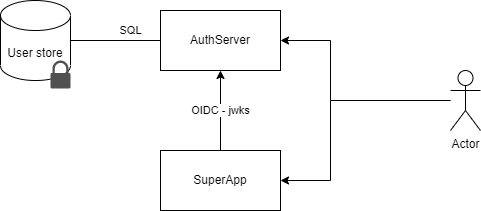
\includegraphics[scale=0.65]{architecture/initial.png}
  \caption{Initial system architecture}
  \label{fig:sys-highlevel}
\end{figure}


\paragraph{Initial state}

In figure \ref{fig:sys-highlevel} we see a high-level overview of a system we are trying to integrate eID authentication. This system consists of the following components:

\begin{enumerate}
  \item AuthServer - the company's SSO; acts as a central authority for identity. Issued OIDC id tokens, which contain user ID, their roles, and claims.
  \item SuperApp - a resource server with access control enabled. It uses id tokens issued by AuthServer and verifies them using asymmetric cryptography.
  \item User store - a data store containing user login information - usernames, password hashes, other PII.
  \item Actor - a physical person accessing the resources in the system.
\end{enumerate}

\paragraph{Desired state}

The company wishes to implement eID authentication. Since the authentication is not done locally but is delegated to some remote service or device, the protocol can be treated as an external federated sign-in. Frameworks such as ASP.NET Identity have special helpful tools to handle external identity providers.

With the inclusion of an external eID provider, we can see the new system architecture in figure \ref{fig:sys-highlevel-witheid}.

\begin{figure}
  \centering
  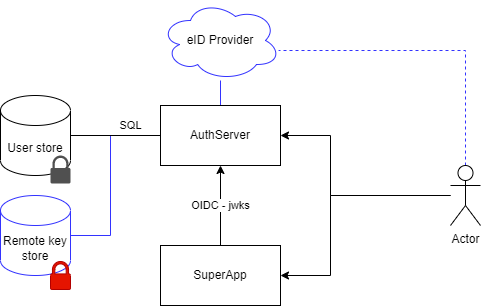
\includegraphics[scale=0.65]{architecture/witheid.png}
  \caption{System architecture after the inclusion of an eID provider}
  \label{fig:sys-highlevel-witheid}
\end{figure}

We can see two significant additions:

\begin{enumerate}
  \item eID provider - a gateway to obtain someone's eID. It can be any eID source like Dokobit, TARA, Smart-ID, ID card.
  \item Remote key store - it is a storage for unique identifiers provided by the eID provider.
\end{enumerate}

The primary purpose of the remote key store is to link the user ID used in the internal system with the unique identifier provided by the eID provider. Because the unique identifier can change or the same physical person can have multiple eIDs \cite{eidas-saml}, it is required to allow numerous eIDs to map to a single internal ID.

The key store is represented with the addition of a red lock. Depending on the country, the data stored there may be subject to strict privacy regulations. Companies should consider implementing strict access control for this part of the infrastructure.

\paragraph{Final state}

The end goal for the scope of this thesis is to implement three eID providers into the architecture. For normal companies, it would make sense to implement multiple in case they would like to get more coverage. Additionally, they could register non eID providers, such as Google or Microsoft social logins. The final high-level overview of the system can be seen in figure \ref{fig:sys-highlevel-final}.

\begin{figure}
  \centering
  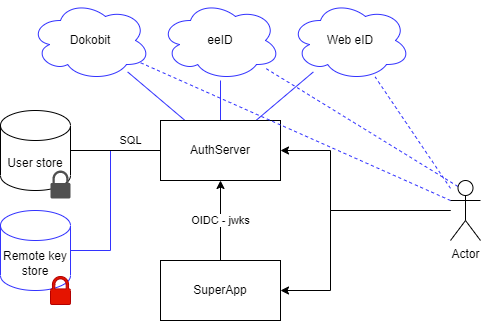
\includegraphics[scale=0.65]{architecture/final.png}
  \caption{System architecture after the inclusion of all eID providers in scope}
  \label{fig:sys-highlevel-final}
\end{figure}

\subsubsection{Process overview}

For validation of the architecture, we will consider two use cases.

The first one (see figure \ref{fig:sysprocess-a}) is concerned about accessing a protected resource with a token issued by the AuthServer. This use case validates the base state of the system.

The second use case (see figure \ref{fig:sysprocess-b}) is also concerned about accessing a protected resource, but only those, who authenticate with a higher level of assurance, like eID, can access it. This use case validates the successful implementation of eID authentication and access control.

\begin{figure}
  \centering
  \begin{sequencediagram}
    \newthread{A}{Actor}{}
    \newinst[3]{B}{AuthServer}{}
    \newinst[1]{C}{SuperApp}{}

    \begin{call}{A}{accessProtected()}{C}{401 Unauthorized}\end{call}

    \begin{call}{A}{authWithPassword()}{B}{Auth token}\end{call}
    \begin{call}{A}{accessProtected()}{C}{Data}\end{call}
    \begin{call}{A}{accessReallyProtected()}{C}{403 Forbidden}\end{call}
  \end{sequencediagram}
  \caption{System behavior when authenticated with a username + password scheme}
  \label{fig:sysprocess-a}
\end{figure}

\begin{figure}
  \centering
  \begin{sequencediagram}
    \newthread{A}{Actor}{}
    \newinst[2]{B}{AuthServer}{}
    \newinst[1]{C}{SuperApp}{}

    \begin{call}{A}{accessProtected()}{C}{401 Unauthorized}\end{call}

    \begin{call}{A}{authWithEid()}{B}{Auth token}\end{call}
    \begin{call}{A}{accessProtected()}{C}{Data}\end{call}
    \begin{call}{A}{accessReallyProtected()}{C}{Very Secret Data}\end{call}
  \end{sequencediagram}
  \caption{System behavior when authenticated with an eID scheme}
  \label{fig:sysprocess-b}
\end{figure}

\subsubsection{Linking eID to an internal user ID}

There will be a need to uniquely link an identity to an internal account in the company SSO. The security requirement, in this case, is not to allow other users to access the same account. For this goal, companies must use one or more person-identifying properties.

When using a passport as a reference, it has the following identifiers: (issuer) country code, document number, surname, given name, personal code, citizenship, date of birth, date of issue, date of expiry, and authority. In these cases, it is easy to use the personal code for identifying a person as it is unlikely to change - people change names, documents expire; authorities and date of birth do not narrow it down nearly enough.

Implementers will hit a roadblock when checking a passport of Ireland - additionally, it has a place of birth but, more importantly, no personal identification code. In this case, the next best unique identifier would be to use the document number and update the account with a new number when the document eventually expires and is replaced.

In the world of digital identity, the eIDAS node network must provide a unique identifier for all requests \cite{eidas-saml}. Having a standardized way of obtaining an identifier is good news. All countries who wish to connect to the eIDAS network would have to expose some code to identify a person uniquely, removing the burden from the software architects to analyze what identifier they should use.

In the eIDAS node network, the unique identifier remains "unchanged for the lifetime of the account" \cite{eidas-saml}. Unfortunately, it does not mean that identifiers cannot change; the account associated with that identifier cannot change. If an identifier were to change when "the user's digital identity is replaced or repaired," relying parties should treat the newly obtained identifier as a completely new identity.

\paragraph{eIDAS Unique Identifier Structure} In eIDAS SAML Attribute Profile, an identifier code is defined as:
\begin{enumerate}
  \item The first part is the Nationality Code of the identifier. This is one of the ISO 3166-1 alpha-2 codes, followed by a slash ("/")).
  \item The second part is the Nationality Code of the destination country or international organization. This is one of the ISO 3166-1 alpha-2 codes, followed by a slash ("/").
  \item The third part is a combination of readable characters. This uniquely identifies the identity asserted in the country of origin but does not necessarily reveal any discernible correspondence with the subject's actual identifier (for example, username, fiscal number etc).
\end{enumerate}

Example: ES/AT/02635542Y (Spanish eIDNumber for an Austrian SP).

\paragraph{Summary} Using eIDAS Unique Identifier structure as a base, we can see that it is enough to uniquely identify a digital identity in eIDAS with the country of origin, country of destination, and a set of characters to identify that person in the origin country. The destination country will always be the same in our company's case. To uniquely identify a person, we will only need its origin country and a unique identifier a member state must provide.

For this thesis, identifiers will be marked as "{\{ISO 3166-1 alpha-2\}}/{\{Code provided by country\}}". Unique identifier examples: EE/38001085718, LT/49003111045, SE/870314-2391.

\subsubsection{Privacy Policy}

The company wishing to implement eID authentication will have to deal with personal information as described by GDPR \cite{eulaw-gdpr}. Before going live with an eID solution, companies must first consult a legal professional for advice.

A privacy policy is a legal document and is way outside of the scope of a technical implementation thesis. However, it is still important to understand the basics. For this goal, two privacy policies will be analyzed: Web eID \cite{legal-webeid-privacypolicy} and Dokobit \cite{legal-dokobit-privacypolicy}.

From the cursory analysis of the two policies, there are three fundamental aspects our company needs to address: what data is processed, with whom the company shares the data, and what is the retention policy.

Based on the privacy policies of Web eID and Dokobit, we constructed a rudimentary privacy policy for the use of the test application environment. A copy of the text can be found in the thesis' appendices.

Further research can be done to outline better the GDPR requirements needed to process a person's eID.

\subsection{Weak points in the architecture}
\subsection{Case Study: Dokobit}
\subsection{Case Study: eeID}
\subsection{Case Study: Web eID}

\subsubsection{About}

Released in the Summer of 2021 \cite{ria-webeid} and having undergone significant changes in January of 2022, this eID framework allows users to authenticate and sign documents using their smart cards.

Functionally this framework is split into three parts: software the user needs to install on their computer, a javascript library that acts as a data intermediary, and the certificate validation library for the back-end.

The software users need to install is similar to the one various countries' governments issue. The significant difference is that this software supports more than one countries' eID solutions. Supported countries include Estonia, Latvia, Lithuania, and Finland \cite{ria-webeid}.

\subsubsection{Data Flow}

Figure \ref{fig:web-eid-authentication} displays the high-level overview of the complete flow of data within the Web eID framework. A detailed explanation of the steps can be found on the technical specification page \cite{ria-webeid-systemarchitecture}. Companies implementing the framework should only consider the browser and the server application (steps 1-3 and 13-17).

\begin{figure}
  \centering
  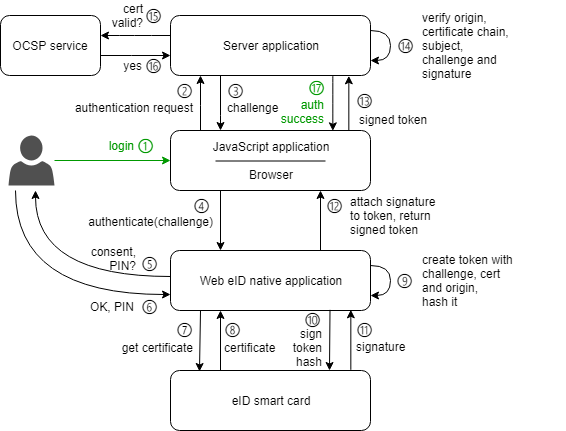
\includegraphics[scale=0.6]{webeid/Web-eID-authentication-communication-diagram}
  \caption{Web eID Authentication flow \cite{ria-webeid-systemarchitecture}}
  \label{fig:web-eid-authentication}
\end{figure}


\subsubsection{Security Analysis}

Researcher Arnis Paršovs published a security analysis of the protocol v1 in October of 2021 \cite{arnis-report-webeid}. Developers behind the Web eID framework acknowledged the weaknesses and addressed them in v2 \cite{ria-webeid-systemarchitecture}, which will be used in the scope of the thesis. At the time of writing, independent researchers and auditors have not yet performed security analysis for this version.

\paragraph{Actors}

The actors in the figure \ref{fig:eid-auth-flow-seq} assume the roles of: QSCD Interface - web-eid.js \cite{ria-webeid-source-web-eid-js}, web-eid-app \cite{ria-webeid-source-web-eid-app}; QSCD - Smart cards of Estonia, Latvia, Lithuania, and Finland \cite{ria-webeid}.

Even though distributed by the same website, id.ee, this interface is separate from the official id.ee software Estonian citizens use to sign and verify documents. "In the future, the final version of Web eID will be added into the ID-software installation package, available for the users the website on www.id.ee" \cite{ria-webeid}. Owners of other countries' smart cards will still have to download the special software from id.ee.

\paragraph{Threat protection}

The Web eID framework uses an insecure channel for communications, so developers must take caution and verify received data when implementing the framework.

Unlike in the cases of Dokobit and eeID, the risk of impersonation is not transferred to the eID service provider.

\TODO{Discussion: suggest how the certificates are way too challenging to obtain for a casual company and may lead to additional vulnerabilities}
\TODO{Discussion: phishing attacks if the company establishes policy to add certificates if they cannot sign in with their card}

\subsubsection{Trust Anchor}

Unlike Dokobit and eeID, Web eID does not provide any guarantees about the trustworthiness of a certificate. It is, however, not out of malice and reminds developers by sending the certificate in a field called "unverifiedCertificate" \cite{ria-webeid-source-web-eid-authtoken-validation-java-readme}.

The relying party must verify the certificate and challenge themselves by checking the origin, certificate expiry, trust chain, OCSP response, and the challenge. This validation structure makes the trust anchor technological and highly dependent on the implementation correctness by the developers.

\todo{Discuss how we can never trust developers without proper supervision}

\subsubsection{Pricing}

The Web eID authentication service is free of charge, as the only external validation, OCSP \cite{rfc6960} requests are free to use. When creating digital signatures, the timestamping service may require payment \cite{ria-webeid-source-web-eid-authtoken-validation-java-readme}.

\subsubsection{Implementation}

For each protocol implementation step, developers will have to fulfill certain guarantees before the system goes into production.

\paragraph{Steps 1-3}

Building the challenge nonce. The goal of these steps is to create the challenge the user will have to sign with their private key. There are a couple of guarantees the application must provide:
\begin{enumerate}
  \item Generated challenge nonce must be between 32 and 96 bytes (inclusive) in length \cite{ria-webeid-source-web-eid-app-authenticate};
  \item "It must be guaranteed that the authentication token is received from the same browser to which the corresponding challenge nonce was issued" \cite{ria-webeid-source-web-eid-authtoken-validation-java-readme}. The framework creators suggest attaching it to the user session.
  \item "Cache must be used for protection against replay attacks by guaranteeing that each authentication token can be used exactly once" \cite{ria-webeid-source-web-eid-authtoken-validation-java-readme}.
  \item "Cookie-based authentication must be protected against cross-site request forgery (CSRF) attacks and extra measures must be taken to secure the cookies by serving them only over HTTPS and setting the HttpOnly, Secure and SameSite attributes" \cite{ria-webeid-source-web-eid-authtoken-validation-java-readme}.
\end{enumerate}

In the implementation example, these measures were addressed by:
\begin{enumerate}
  \item a 64 byte cryptographically secure randomly generated nonce is created (see listing \ref{lst:web-eid-challenge});
  \item challenge nonce is set in the user's session, which adversaries cannot tamper;
  \item the generated nonce is stored into local memory cache for later use; nonce expires after 5 minutes;
  \item an input field is rendered on the page with a unique CSRF validation token, which prevents cross-site request forgery attacks (see listing \ref{lst:web-eid-challenge-ui});
\end{enumerate}

\begin{lstlisting}[caption={Web eID Challenge Endpoint}, label={lst:web-eid-challenge}]
private TimeSpan ChallengeLifetime { get; } = TimeSpan.FromMinutes(5);

private readonly IMemoryCache _cache; // Injected

[HttpGet("challenge")]
public IActionResult GetChallenge()
{
    var nonce = RandomNumberGenerator.GetBytes(64);

    _cache.Set(Convert.ToBase64String(nonce), true, ChallengeLifetime);
    HttpContext.Session.Set("eid.challenge", nonce);

    return Ok(new { nonce });
}
\end{lstlisting}


\begin{lstlisting}[caption={Web eID UI excerpt}, label={lst:web-eid-challenge-ui}, language={html}]
@inject Microsoft.AspNetCore.Antiforgery.IAntiforgery _csrf
@{ var csrfToken = _csrf.GetAndStoreTokens(HttpContext); }

<!-- Button used to sign in -->
<a role="button" class="btn btn-secondary" id="webeid-auth-button">Web eID</a>

<input id="csrfToken" type="hidden" value="@csrfToken.RequestToken"/>

<script>
    ...

    const authTokenResponse = await fetch("/signin-id/login", {
        method: "POST",
        headers: {
            "Content-Type": "application/json",
            "RequestVerificationToken": document.getElementById("csrfToken").value
        },
        body: JSON.stringify(...)
    });

    ...
</script>
\end{lstlisting}

\paragraph{Steps 13-17}

After the user signs the nonce challenge and sends their certificate, the server must verify its authenticity. The application must perform all of the following before allowing the user to sign in:

\begin{enumerate}
  \item verify the CSRF token from earlier steps \cite{ria-webeid-source-web-eid-authtoken-validation-java-readme};
  \item verify the challenge nonce came from the original user and has not expired, was not consumed;
  \item verify the certificate validity and check if nonce was signed by the associated private key (see below);
  \item issue an authentication token with the fields from the certificate's subject;
\end{enumerate}

In the implementation example, these measures were addressed by:
\begin{enumerate}
  \item the back end endpoint for login is decorated with ValidateAntiForgeryToken Attribute. This attribute instructs the ASP.NET API to ignore requests not containing a CSRF token \cite{msdocs-anti-request-forgery}. A JavaScript application can only access the protected endpoints by providing RequestVerificationToken header (see listing \ref{lst:web-eid-challenge-ui});
  \item the application tries to extract the challenge nonce from the browsing session. The process would succeed if the session cookie were not modified. After the extraction, the application checks the nonce cache to verify if the challenge is still active. Cache hit means the nonce has not expired, and no previous authentication attempt was performed. Remove the challenge nonce from all stores.
  \item The API calls a standalone validation service to verify the nonce and certificate (see below).
  \item Application populates the ASP.NET identity management system with the fields from the certificate: serial number, given name, surname, country. An identity session cookie is sent to the client.
\end{enumerate}

\begin{lstlisting}[caption={Web eID Login Endpoint}, label={lst:web-eid-login}]
[HttpPost("login")]
[ValidateAntiForgeryToken]
public async Task<IActionResult> Login([FromBody] WebIdAuthTokenResponse token)
{
    // Obtain the challenge from session
    if (!HttpContext.Session.TryGetValue(ChallengeNonceKey, out var nonce) && nonce == null)
        return Unauthorized();

    // Check if token was not used before or expired
    var challenge = Convert.ToBase64String(nonce);
    if (!_cache.TryGetValue(challenge, out _))
        return Unauthorized();

    _cache.Remove(challenge);
    HttpContext.Session.Remove(ChallengeNonceKey);

    // Validate the certificate and signed challenge
    var validationResult = await _webEidValidationService.GetResult(new WebEidValidationRequest(token, nonce));
    if (!validationResult.Success)
        return Forbid();

    // Certificate is valid. Sign in the user

    await HttpContext.SignInAsync(BuildUser(new X509Certificate2(Convert.FromBase64String(token.UnverifiedCertificate)).Subject));

    return Ok();
}
\end{lstlisting}

\paragraph{Certificate and nonce verification}

This step is the most complicated in the entire validation process. To prevent any issues with incorrect implementation, the framework maintainers recommend using their library for validation \cite{ria-webeid-source-web-eid-authtoken-validation-java-readme}. Libraries can come with security vulnerabilities, and developers are reluctant to update their used version; however, it is still more favorable to creating vulnerabilities from misconfiguration \cite{9240619}.

The eu.webeid.security Java package performs most of the certificate validation: expiry, purpose, policy, OCSP \cite{ria-webeid-source-web-eid-authtoken-validation-java-readme}. Developers will only have to configure the CA and host validation. Configuration is handled by providing a set of trusted CA certificates for trust chain verification and the hostname for challenge nonces (see listing \ref{lst:web-eid-java-lib}).

\todo{This library does favor EE cards a lot more, even having hardcoded some Mobile ID policies. Not sure if it is worth mentioning.}

\begin{lstlisting}[caption={Web eID Login Endpoint}, label={lst:web-eid-java-lib}]
public class AuthTokenValidatorService {

  @Bean
  public AuthTokenValidator validator() {
    try {
      return new AuthTokenValidatorBuilder()
        .withSiteOrigin(URI.create(System.getenv("ORIGIN_URL")))
        .withTrustedCertificateAuthorities(loadTrustedCACertificatesFromCerFiles())
        .build();
    } catch (JceException e) {
      throw new RuntimeException("Error building the Web eID auth token validator.", e);
    }
  }

  private X509Certificate[] loadTrustedCACertificatesFromCerFiles() {
    List<X509Certificate> caCertificates = new ArrayList<>();

    try {
      CertificateFactory certFactory = CertificateFactory.getInstance("X.509");

      File[] files = new File("/certs").listFiles((f, n) -> n.endsWith(".cer"));
      if (files != null) {
        for (File file : files) {
          try (InputStream stream = new FileInputStream(file)) {
            X509Certificate caCertificate = (X509Certificate) certFactory.generateCertificate(stream);
            caCertificates.add(caCertificate);
          }
        }
      }
    } catch (CertificateException | IOException e) {
      throw new RuntimeException("Error initializing trusted CA certificates.", e);
    }

    return caCertificates.toArray(new X509Certificate[0]);
  }
}
\end{lstlisting}

The token validation service described in listing \ref{lst:web-eid-java-lib} requires the maintainers to set the origin URL in the form of an environment variable and to populate the folder {/certs} with trusted CA certificates.

Origin URL can be obtained by checking the {window.origin} JavaScript variable in the page containing the sign-in button.

For the CA certificate set, the company can get an up-to-date list of trusted certificates at the EU Trust Services Dashboard \cite{eu-trustservices}. The issue with this list is that it contains all trust certificates for various scopes. In our case, we should limit the search to the extent of QCert for ESig. In the case of Estonia and Lithuania, only three entities are certified to issue certificates for QSCD (see figure \ref{fig:eu-tsp-list}). It is in stark contrast to Spain's 31 \cite{eu-trustservices}. It is possible to further narrow down to only certificate generation services for qualified certificates (CA/QC).

\begin{figure}
  \centering
  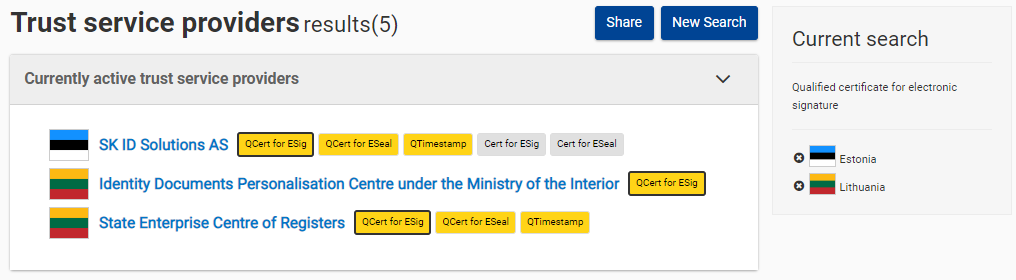
\includegraphics[scale=0.54]{webeid/eu-tsp-search}
  \caption{List of EU Trust service providers of Estonia and Lithuania capable of creating qualified certificates for e-signatures}
  \label{fig:eu-tsp-list}
\end{figure}

In the case of Estonia's single TSP, we can see that only 3 CA are currently operational (see figure \ref{fig:eu-tsp-skid}). Unfortunately, there is no standardized way of narrowing down which certificates could be used for authentication.

\begin{figure}
  \centering
  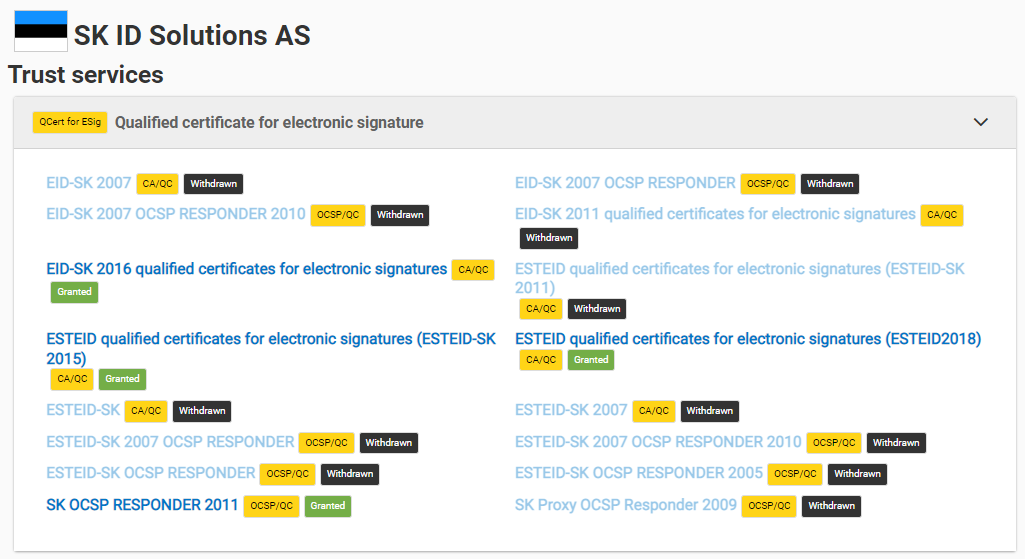
\includegraphics[scale=0.54]{webeid/eu-tsp-skid}
  \caption{List of certificates issued to SK ID Solutions AS for the purposes of Qualified certificate for electronic signature}
  \label{fig:eu-tsp-skid}
\end{figure}

An alternative way to obtain certificates would be to go to the government authority of each country responsible for the distribution of certificates. This action requires prior knowledge of who is responsible for issuing certificates and their purposes.

In Lithuania's case, it is the Ministry of the Interior \cite{eid-lt-ministryofinterior-certificates} who issue two certificates (A and B) every couple of years. As of early 2022, four certificates are active, and all will be added to the trusted CA list.

In Estonia's case, SK ID Solutions manages the CA certificates \cite{eid-ee-skid-certificates}. Of the three certificates found on the EU Trust Services Dashboard, only two are relevant to us, the 2015 and 2018 ones, as the 2016 one has its purpose for use in Smart-ID, which the Web eID framework does not support.

The final list of certificates to support Lithuania and Estonia include four certificates from Lithuania's Ministry of the Interior and two certificates issued by SK ID Solutions for a total of six. It is essential to keep track of these certificates as each one of them can act as a point of compromise and must be monitored in the event they are revoked for security \cite{roca-vulnerability-lessons-learned} or other issues.

\paragraph{Exposing the service}

With the certificate validation service configured, it is now required to link it to the Web API. If the company orients around using microservices, this service can be just that. All that the validation service requires is to expose an endpoint that accepts a nonce and a token from the javascript library and returns a validation result.

Companies must take proper measures to protect such service from adversaries as it acts as a fundamental trust anchor. Developers should take steps outlined in assume breach \todo{citation missing} to mitigate the risk of misuse.

\TODO{Related research about legal person documents?}

\TODO{High-level overview of the system}
\TODO{Points of compromise?}
\TODO{Complete alternative, using your own issued certificates?}
\section{Discussion}

\subsection{Do businesses even want eID?}

When conducting the initial investigation on what criteria we should use to compare different eID providers, we interviewed the CTO of a logistics company. The full interview can be found in the appendix. The responses about current practices were shocking but not surprising.

\paragraph{Authentication or Digital Signatures. What is more important to you?}

When asked if there was a choice between implementing eID authentication and qualified digital signature infrastructure, the company's focus would be on digital signature. Authentication only helps ensure the confidentiality and integrity of data and requires an additional heap of technological measures to prevent bypass. Qualified digital signatures offer an immediate benefit in the form of legally binding documents.

\paragraph{Trust. What trust requirements the eID provider should fulfill for you to adopt it?}

When asked if ISO/IEC 20001:2013 certification is sufficient, the answer was a resounding no. This certification should be the bare minimum for the company to consider using that solution. The CTO would "like to see that government portal, or banks are adopting this solution. This provides sufficient trust into the solution". This quote supports the assumption at the start that widespread adoption is low because there are no big-name adopters.

\paragraph{Source. Does the eID have to come from a TSP?}

The company CTO was not concerned much about the kind of eID provider is: primary or third-party. As long as other large entities the solution is trusted by other entities (governments or large companies), there is no significant difference between choosing services from an eIDAS QTSP and not. This logistics company sees no clear advantage in creating a contract with SK ID Solutions to implement Smart-ID authentication over an agreement with the Estonian Internet Foundation.

One can argue that a TSP is the trusted solution by large governmental institutions; however, it comes with a problem, especially in Estonia, of poor market reach, which is also highly important.

\paragraph{Market reach. How much impact does it have?}

While trust and security in solution are the main deciding factors, increasing security would not attract companies to use an eID solution after it reaches a certain widespread adoption level. What will have more impact is the market reach.

We have presented the interviewee four options: eeID (eIDAS), Dokobit (private company), Web eID (DIY), Smart-ID (narrow specialty TSP). With all their advantages and disadvantages, assuming all reach the trust requirement and price of operations are similar, the CTO's option was the one with the highest market reach. The reasoning behind it was saving money on implementing multiple providers, and the less company has to do, the lower the risk of something going wrong.

In short, a larger market size would positively impact the decision process of choosing a particular eID provider.

\paragraph{Pricing. How much is worth spending on eID solutions?}

Reducing costs is one of the cornerstones of running a business. When presented with the ballpark of how much the company would have to spend to operate an eID solution, the company's CTO suggested looking at the broader market for identity management solutions. They currently use Azure for their services. The company would still need to pay Microsoft for their accounts to access the cloud platform infrastructure. Azure AD B2C is used for all other use cases, which provides identity management options the company is used to, and the operational cost is close to nothing.

The issue with the eID solutions is that they are targeting a different kind of company. Still, it is not clear which industry would willingly, without regulatory requirements, choose to implement such a system. The CTO estimates that for 10 000 authentications per month, a company could reasonably support 300-400 active users. This price effectively means adding 1€ per system user to operational costs. Not many industries can afford such a luxury.

\paragraph{Technological hurdles}

The system is only as secure as its weakest link. The hardest part of implementing an eID solution is not integrating with an external provider but creating access controls for new or existing resources. These measures will have to be in place for all interaction methods - from user interfaces to database and backup solutions.

\paragraph{Summary}

Ultimately, the eID authentication solution suffers from a lack of benefits for companies. This solution deals with authentication and, by extension, access control. There is no visible advantage of using eID over a regular MFA solution from Microsoft. The company is just not dealing with data that personal.

The picture I have painted from the interview is that for the eID authentication to be helpful, there should be a legitimate interest to obtain the user's national ID code. There are cheaper alternatives available for those interested in only the additional security measures.

\subsection{Do businesses even want digital signatures?}

If there is one quote to take from the interview, it must be "today [business owners] open PDF and apply PNG of signature into the file free of charge." Part of the reason why eID authentication is not widespread is that digital signatures are not widespread.

The benefits of eID in the private sector, even after the research, remain unclear. The value provided by Qualified Electronic Signatures is obvious.

The only real business value eID authentication provides - is trustworthy audit logs in the case of legal disputes. Still, even then, there are no high-profile cases in court on that matter. Although, it would be harder for defendants to claim they didn't access the system when logs clearly showed. Unfortunately, even that argument collapses when you look at the trust chain - people in power can sabotage AuthServer, issue tokens in the victim's name, fabricate access records.

The only thing that is legally binding is Qualified Digital Signatures. Only special approved devices can create digital signatures, and when signing, the cryptographic operations are performed on the device. There is no higher authority like AuthServer that can doctor these signatures.

Unfortunately, even with the visible advantages of electronic signatures, business owners still do not use them. Having a picture of a written signature inside a PDF document remains a popular way of doing business.

\TODO{Talk about which of the 3 case studies would work best in a company in early 2022}
\todo{Should notify how eeID and Web eID are really in their infancy and further research should repeat this study in a couple of years}

\subsection{Which eID provider to choose?}

The three case studies were not selected at random, they represent different approaches to accessing the electronic identity. Summary of pros and cons can be seen in table \ref{tab:eid-advantages-disadvantages}.

\begin{table}[h]
    \centering
    \caption{Advantages and disadvantages of each eID solution}
    \begin{tabular}{p{2cm} | p{2cm} | p{4.4cm} | p{4.4cm}}
        \bf{Scheme}            & \bf{Examples}                           & \bf{Advantages}                                                                                                                                                          & \bf{Disadvantages}                                                                                                             \\
        \hline
        eIDAS                  & TARA, (eeID)                            & large target audience; \newline officially supported and used by governments; \newline cheaper than implementing many individual QTSP services;                          & may not include some more popular schemes; \newline does not offer means to sign documents;                                    \\
        \hline
        Third-party aggregator & Dokobit, Signicat, (eeID), (Web eID)    & large target audience; \newline includes schemes excluded from eIDAS; \newline cheaper than implementing many individual QTSP services;                                  & not officially supported by governments or legislation; \newline trust issues; \newline risk of provider ceasing operations;   \\
        \hline
        QTSP                   & ID-Card, Mobile-ID, Smart-ID, (Web eID) & highest degree of trust; \newline security audits are regulated by law; \newline support for digital signatures; \newline some options (ID card) can be free to operate; & very narrow market reach in comparison; \newline complicated to integrate; \newline paid service operational stack up quickly; \\
    \end{tabular}
    \label{tab:eid-advantages-disadvantages}
\end{table}

\paragraph{Which to choose?} First, companies should decide if they need eID authentication in the first place. After that, it depends on priorities.

If the highest degree of trust factor is required, a company will have no other option other than to use a QTSP.

If high market reach and stability are required, adequately vetted and audited eIDAS node access is likely to be the best choice.

If the highest market reach is everything, third-party providers are a great choice. They are separated from the eIDAS category because they can use digital authentication schemes the origin countries do not wish to be liable for.

In short, there is no clear advantage of one option over the other, and companies should address the options available to them individually.

\TODO{Footnote on ID generation. Why not use the id and not store? Generally you would want to store who created a internal document, or who last edited a page. Using national ID for this purpose can open pandoras box when it comes to logging. Pseudonimization and linking the keys behind strong locks is next best thing.}

\subsection{Dangers with having no control over identity}

As per the case with using external identity providers such as Auth0, Azure AD, or AWS Cognito, companies put a significant amount of trust when using their services. These services create access tokens, which almost always contain some form of user-id, roles, or claims.

From a technical standpoint, nothing stops these companies from creating fake access tokens skipping the whole authentication process. As far as the relying party would be concerned, these tokens would be indistinguishable from real ones. A corrupt or compromised company would have to only need to compromise the last step of authentication protocol - the one that sends (and optionally signs) personal information.

The same security concerns apply to state-issued electronic identity. We can identify three tiers of security, ordered from most to least secure:

\begin{enumerate}
    \item Local device certificate authentication. Examples include ID cards and USB keys.
    \item Local device certificate authentication. Examples include Mobile-ID and Smart-ID.
    \item Third party authentication. Examples include eeID and Dokobit.
\end{enumerate}

In the example of local device certificate authentication, a weakness lies in the fact that those certificates can be freely generated


\paragraph{Is it likely?} \todo{Does this make sense?}

Ultimately, governments should have no interest in compromising their systems. The only benefit of doing so is simply too contrived - they would gain the ability to frame someone in a heavily audited space to have an edge in court. There are more straightforward legal or technical methods for all other activities.

More importantly, the issue with any system is that if an interaction method exists, it is bold to assume that only the intended users can access it. It is not unreasonable to think that backdoors can themselves have backdoors. Thus the only 100\% safe countermeasure preventing anyone from accessing a system would be to make sure no one can.

In conclusion, it makes little sense for companies or governments to compromise their systems. The risks in doing so are astronomical in comparison to the benefits received.
\section{Conclusion}

In the thesis, we looked into the background, legality, and extensibility of eIDs, discussed the viability of using eID as a replacement for authentication, and analyzed three different eID providers the private sector could implement.

We have shown that it is possible to integrate an eID authentication scheme into a pre-existing SSO easily. The discovered challenges with integration are protecting the data from access by other means - no reason to force users to authenticate with eID if they can access the database with {username and password}.

We have created a privacy policy for the dummy test application considering the privacy requirements imposed by GDPR.

We have compared three different eID providers and discovered three different ways of performing cross-border authentication: integrating each provider individually, integrating a third-party provider aggregator, or tapping into a legally governed eIDAS framework.

We have discovered that all three authentication schemes have had security or integration issues in their protocols, limiting them in some tangible way.

We have interviewed a logistics company representative to gauge the acceptance of eIDs in the general public, only to discover that it is unlikely that companies will adopt this technology without drastic changes in the market.

We have proposed an alternative to eID authentication using a similar scheme when a high certainty behind a given identity is required during enrollment only.

\paragraph{Summary} The ability to integrate eID in the private sector exists; however, the public acceptance of them is limited. The technical and legal challenges associated with eID authentication make it impractical to implement for almost all companies.

% \newpage
% \section{Introduction}

% \TODO{What is it in simple terms (title)?}
% \TODO{Why should anyone care?}
% \TODO{What was my contribution?} 
% \TODO{What you are doing in each section (a sentence or two per section)}

% Tip: if it's hard for you to start writing, then try to split it to smaller parts, e.g. if the title is ``Type Inference for a Cryptographic Protocol Prover Tool'' then the ``What is it'' can be divided into ``what is type inference'', ``what is cryptographic protocol'' and ``what is the prover tool''. These three can also be split to smaller parts etc.




% \newpage
% \section{Title of Section 2} 
% \TODO{Short description of what this section is about}


% \subsection{Title of Subsection 1}

% Some text...

% \subsubsection{Title of Subsubsection 1}

% Some text...

% \subsubsection{Title of Subsubsection 2}

% Some text...



% \subsection{Title of Subsection 2} 

% Rule: If you divide the text into subsections (or subsubsections) then there has to be at least two of them, otherwise do not create any. 

% Tip: You can also use paragraphs, e.g.
% \paragraph{Type rules for integers.} Some text ...

% \paragraph{Type rules for rational numbers.} Some text here too...




% \subsection{How to use references} \label{sec:using_ref}

% \paragraph{Cross-references to figures, tables and other document elements.}
% LaTeX  internally numbers all kind of objects that have sequence numbers:
% \begin{itemize}
% \item chapters, sections, subsections;
% \item figures, tables, algorithms;
% \item equations, equation arrays.
% \end{itemize}
% To reference them automatically, you have to generate a label using \texttt{$\backslash$label\{some-name\}} just after the object that has the number inside. Usually, labels of different objects are split into different namespaces by adding dedicated prefix, such as \texttt{sec:}, \texttt{fig:}. To use the corresponding reference, you must use command \texttt{$\backslash$ref} or \texttt{$\backslash$eqref}. For instance, we can reference this subsection by calling Section~\ref{sec:using_ref}. Note that there should be a nonbreakable space \texttt{\~} between the name of the object and the reference so that they would not appear on different lines (does not work in Estonian).          



% \paragraph{Citations.}
% Usually, you also want to reference articles, webpages, tools or programs or books. For that you should use citations and references. The system is similar to the cross-referencing system in LaTeX. For each reference you must assign a unique label. Again, there are many naming schemes for labels. However, as you have a short document anything works. To reference to a particular source you must use \texttt{$\backslash$cite\{label\}} or \texttt{$\backslash$cite[page]\{label\}}. 

% References themselves can be part of a LaTeX source file. For that you need to define a bibliography section. However, this approach is really uncommon. It is much more easier to use BibTeX to synthesise the right reference form for you. For that you must use two commands in the LaTeX source
% \begin{itemize}
% \item $\backslash$bibliographystyle\{alpha\} or $\backslash$bibliographystyle\{plain\}
% \item $\backslash$bibliography\{file-name\}
% \end{itemize}
% The first command determines whether the references are numbered by letter-number combinations or by cryptic numbers. It is more common to use \texttt{alpha} style. The second command determines the file containing the bibliographic entries. The file should end with \texttt{bib} extension. Each reference there is in specific form. The simplest way to avoid all technicalities is to use graphical frontend  Jabref (\url{http://jabref.sourceforge.net/}) to manage references. Another alternative is to use DBLP database of references and copy BibTeX entries directly form there.   
    
   
% The following paragraph shows how references can be used. Game-based proving is a way to analyse security of a cryptographic protocol~\cite{GameB_1, GameB_2}. There are automatic provers, such as {CertiCrypt\-}~\cite{certicrypt} and ProVerif~\cite{proVerif}.



% \newpage
% \section{How to add figures and pictures to your thesis}


% Here are a few examples of how to add figures or pictures to your thesis (see Figures~\ref{fig:fnCompModel}, \ref{fig:game-based_proofs}, \ref{fig:proveit_screenshot}).

% Rule: All the figures, tables and extras in the thesis have to be referred to somewhere in the text.


% \begin{figure} [ht] %try to place the figure here (next option top of the page) 
% \begin{center}
% 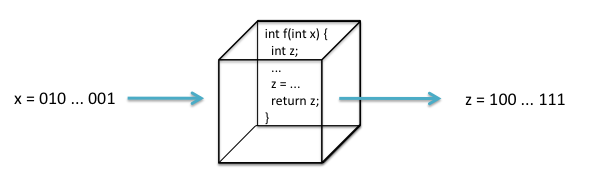
\includegraphics[width=0.8\textwidth]{computational_model_function}
% \caption{The title of the Figure.}
% \label{fig:fnCompModel}
% \end{center}
% \end{figure}



% \begin{figure} [!ht] %if [h] doesn't work, we can force with !
% \begin{center}
% 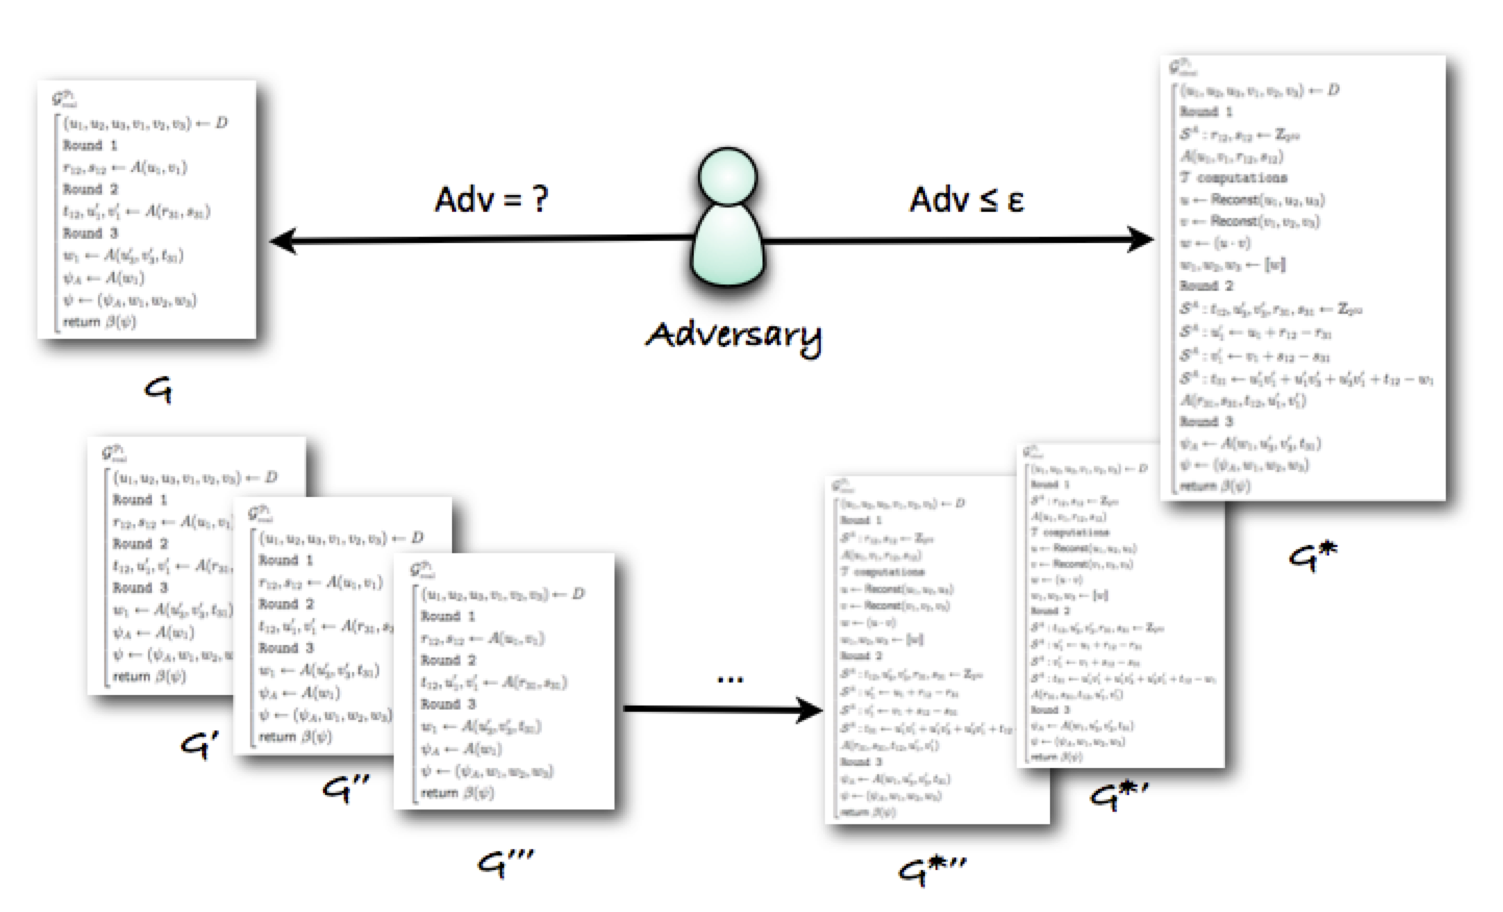
\includegraphics[width=\textwidth]{game-based_proofs}
% \caption{Refer if the figure is not yours~\cite{kamm12}.}
% \label{fig:game-based_proofs}
% \end{center}
% \end{figure}


% \begin{figure} [p]
% \begin{center}
% 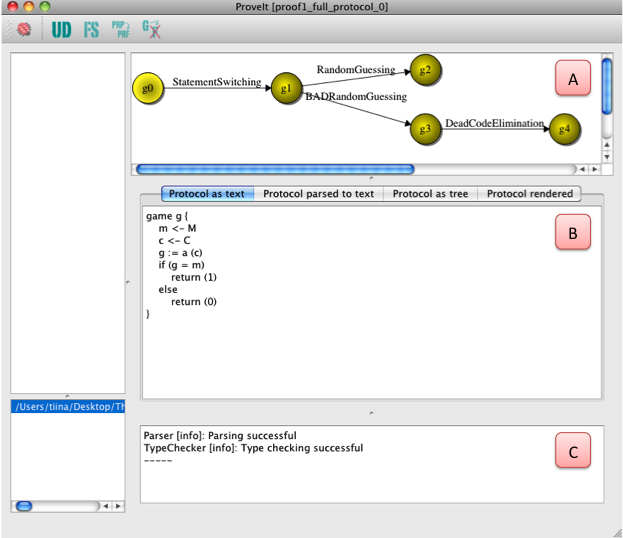
\includegraphics[width=\textwidth]{proveit_screenshot}
% \caption{Screenshot of \proveit.}
% \label{fig:proveit_screenshot}
% \end{center}
% \end{figure}

% Tip: If you add a screenshot then labeling the parts might help make the text more understandable (panel C vs bottom left part), e.g.


% \begin{figure} [htbp]
% \begin{tabular}{c c}
% %
% \begin{minipage}{0.45\textwidth}
% 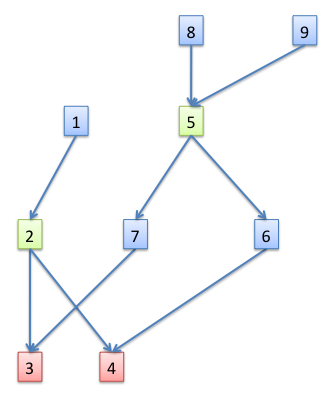
\includegraphics[width=\textwidth]{LCA_2_solutions}
% \end{minipage}
% %
% &
% \begin{minipage}{0.55\textwidth}
% \centering
% \begin{tabular}{ l | l |}
% 	Node & Decendants \\ \hline
%   1 & 2, 3, 4 \\ \hline
%   2 & 3, 4 \\ \hline
%   3 & \\ \hline
%   4 & \\ \hline
%   5 & 3, 4, 6, 7 \\ \hline
%   6 & 4 \\ \hline
%   7 & 3 \\  \hline
%   8 & 3, 4, 5, 6, 7\\ \hline
%   9 & 3, 4, 5, 6, 7\\ \hline
% \end{tabular}
% \end{minipage}
% \end{tabular}
% %
% \caption{Example how to put two figures parallel to each other.}
% \label{fig:LCA_2_solutions}
% \end{figure}


% Example: A screenshot of \proveit can be seen on Figure~\ref{fig:proveit_screenshot}. The user first enters the pseudocode of the initial game in panel B. \proveit also keeps track of all the previous games showing the progress on a graph seen in panel A.

% There are two figures side by side on Figure~\ref{fig:LCA_2_solutions}.



% \clearpage %if newpage doesn't work
% \section{Other Ways to Represent Data}

% \subsection{Tables}

% \begin{table}[h]
% \centering
% \caption{Statements in the \proveit language.}
% \begin{tabular}{| l | l |}
% 	\hline
% 	\bf{Statement} & \bf{Typeset Example} \\
% 	\hline
% 	assignment & $a := 5 + b$ \\
% 	\hline
% 	uniform choice & $m <- M$ \\
% 	\hline
% 	function signature & $f : K \times M -> L$\\
% 	\hline
% \end{tabular}
% \label{tab:statements}
% \end{table}


% \subsection{Lists}

% Numbered list example:
% \begin{enumerate}
% 	\item item one; 
% 	\item item two;
% 	\item item three.
% \end{enumerate} 

% \subsection{Math mode}
% Example:
% \begin{equation}
% a + b = c + d
% \end{equation}
% Aligning:
% \begin{align*}
% 	a &= 5 \\
% 	b + c &= a \\
% 	a -2*3 &= 5/4
% \end{align*}
% Hint: Variables or equations in text are separated with \$ sign, e.g. $a$, $x - y$.

% \paragraph{Inference Rules}
% \[ 
% 	\inference[addition]{x : T & y : T}{x + y : T} 
% \]
% Bigger example:
% \[
% \inference[assign]{c := a + b & 
% 	\inference[addG]{a : \typeRat & 
% 		\inference[var]{b : \typeInt & \typeInt \subseteq \typeRat}{b : \typeRat}
% 		}{a + b : \typeRat}
% 	}{c : \typeRat}
% \]


% \subsection{algorithm2e}

% \begin{algorithm} [!h]
% 	\caption{typeChecking} \label{alg:typeChecking}
% 	\KwIn{Abstract syntax tree}
% 	\KwResult{Type checking result; In addition, type table \typeF{type\_G} for global variables, \typeF{game} for the main game and \typeF{fun} for each $fun \in F$}
% 	\SetKwData{s}{s}
% 	\BlankLine
	
% 	\While{something changed in last cycle}{
% 		\lForEach{global statement \s} {
% 			\parseStatement{\s, \typeF{type\_G}}\;
% 		}
% 		\ForEach{function $fun$} {
% 		\lForEach{statement \s in $fun$} {
% 			\parseStatement{\s, \typeF{fun}}\;
% 		}
% 		}
% 		\lForEach{statement \s in game} {
% 			\parseStatement{\s, \typeF{game}}\;
% 		}
% 	}
% 	%\eIf{error messages were found}{\Return \False\;}{\Return \True\;}
% \end{algorithm}

% \subsection{Pseudocode}

% \begin{figure} [htb]
% \begin{lstlisting}
% expression
%   : NUMBER
%   | VARIABLE
%   | '+' expression
%   | expression '+' expression
%   | expression '*' expression
%   | function_name '(' parameters ')'
%   | '(' expression ')'
% \end{lstlisting}
% \caption{Grammar of arithmetic expressions.}
% \label{fig:parser_exp}
% \end{figure}

% \subsection{Frame Around Information}

% Tip: We can use minipage to create a frame around some important information.
% \begin{figure} [h]
% \frame{
% \begin{minipage}{\textwidth}
% \begin{enumerate}
% 	\item integer division ($\opDiv$) -- only usable between \typeInt types
% 	\item remainder ($\%$) -- only usable between \typeInt types
% \end{enumerate}
% \end{minipage}
% }
% \caption{Arithmetic operations in \proveit revisited.}
% \label{fig:aritmOp_revisit}
% \end{figure}



% \clearpage
% \section{Conclusion}

% \TODO{what did you do?} 
% \TODO{What are the results?}
% \TODO{future work?}

\newpage

% BibTeX bibliography
\bibliographystyle{unsrt} %plain=[1], alpha=[BGZ09]
\bibliography{unitartucs-thesis}

\addcontentsline{toc}{section}{\refname}


% Use Biblatex if you have problems with Estonian keywords
%\printbibliography %biblatex


% Use alternative local LaTeX bibliography
% \begin{comment}
% \begin{thebibliography}{9}
% \bibitem{proVerif} 
%   Bruno Blanchet. 
%   Proverif: Cryptographic protocol verifier in the formal model.
%   \url{http://www.proverif.ens.fr/}.
%   (checked 15.05.2012)
% \bibitem{GameB_1} GameB1
% \bibitem{GameB_2} GameB2
% \bibitem{certicrypt} certicrypt
% \bibitem{kamm12} kamm12
% \end{thebibliography}
% \end{comment}


\section*{Appendix}
\addcontentsline{toc}{section}{Appendix}

\section*{I. Glossary}
\addcontentsline{toc}{subsection}{I. Glossary}
%=== Licence in English
\newcommand{\licencehint}[2]{\\\hspace*{#1}\textsl(#2)\par}
\newcommand\EngLicence{{%
\selectlanguage{english}
\section*{V. Licence}

\addcontentsline{toc}{subsection}{V. Licence}

\subsection*{Non-exclusive licence to reproduce thesis and make thesis public}

I, \textbf{Gediminas Milašius}, %author's name

\begin{enumerate}
\item
herewith grant the University of Tartu a free permit (non-exclusive licence) to reproduce, for the purpose of preservation, including for adding to the DSpace digital archives until the expiry of the term of copyright,
\par
\textbf{Integration analysis of various eID authentication solutions used in the private sector of Estonia}, %
supervised by Arnis Paršovs. %supervisor's name
\item
I grant the University of Tartu a permit to make the work specified in p. 1 available to the public via the web environment of the University of Tartu, including via the DSpace digital archives, under the Creative Commons licence CC BY NC ND 3.0, which allows, by giving appropriate credit to the author, to reproduce, distribute the work and communicate it to the public, and prohibits the creation of derivative works and any commercial use of the work until the expiry of the term of copyright.
\item
I am aware of the fact that the author retains the rights specified in p. 1 and 2.
\item
I certify that granting the non-exclusive licence does not infringe other persons' intellectual property rights or rights arising from the personal data protection legislation. 
\end{enumerate}

\noindent
Gediminas Milašius\\ %author's name
\textbf{\textsl{2022-05-10}}
}}%\newcommand\EngLicence


%=== Licence in Estonian
\newcommand\EstLicence{{%
\selectlanguage{estonian}
\section*{II. Litsents}

\addcontentsline{toc}{subsection}{II. Litsents}

\subsection*{Lihtlitsents lõputöö reprodutseerimiseks ja üldsusele kättesaadavaks tegemiseks}

Mina, \textbf{Gediminas Milašius}, %author's name
  \licencehint{10mm}{autori nimi}

\begin{enumerate}
\item
annan Tartu Ülikoolile tasuta loa (lihtlitsentsi) minu loodud teose
\par
\textbf{Tüübituletus neljandat järku loogikavalemitele}, %title of thesis
    \licencehint{10mm}{lõputöö pealkiri}
\par
mille juhendaja(d) on Arnis Paršovs, %supervisor's name(s)
  \licencehint{10mm}{juhendaja nimi}
\par
reprodutseerimiseks eesmärgiga seda säilitada, sealhulgas lisada digitaalarhiivi DSpace kuni autoriõiguse kehtivuse lõppemiseni.
\par
\item
Annan Tartu Ülikoolile loa teha punktis 1 nimetatud teos üldsusele kättesaadavaks Tartu Ülikooli veebikeskkonna, sealhulgas digitaalarhiivi DSpace kaudu Creative Commonsi litsentsiga CC BY NC ND 3.0, mis lubab autorile viidates teost reprodutseerida, levitada ja üldsusele suunata ning keelab luua tuletatud teost ja kasutada teost ärieesmärgil, kuni autoriõiguse kehtivuse lõppemiseni.
\item
Olen teadlik, et punktides 1 ja 2 nimetatud õigused jäävad alles ka autorile.
\item
Kinnitan, et lihtlitsentsi andmisega ei riku ma teiste isikute intellektuaalomandi ega isikuandmete kaitse õigusaktidest tulenevaid õigusi. 
\end{enumerate}

\noindent
Gediminas Milašius\\ %author's name
\textbf{\textsl{11.06.2022}}
}}%\newcommand\EstLicence


%===Choose the licence in active language
\iflanguage{english}{\EngLicence}{\EstLicence}
\section*{III. Questionnaire}
\addcontentsline{toc}{subsection}{III. Questionnaire}

This interview's goal is to understand better the reasons for the poor adoption of eIDs in the private sector.

This interview was conducted with the CTO of a multinational logistics company.

\begin{enumerate}
    \item With electronic key cards, users can authenticate themselves using a piece of hardware, say a card or a USB stick. This authentication method is often more secure than the usual username and password approach. Are you and the company in general aware of this?
    
    \textbf{Ashot: yes, fully aware. But you have to keep hardware always with you, besides that it can be lost or stolen. That's why MFA is a preferred way for authentications and it get global adoption.}
    \item I would describe an eID scheme as something like your id card, but digitally. There are three main schemes in Estonia: ID cards, Mobile-ID, and Smart-ID. Are you familiar with at least one of them?
    
    \textbf{Ashot: yes, all of them. Using Mobile-ID and Smart-ID all the time, Smart-ID is somehow more user-friendly. ID card - exceptional cases.}
    \item With the eIDAS regulation, these three eID schemes can create digital signatures with the legal value of a handwritten signature. Do you have a place in the company where you print a document, sign it, scan it and upload it? Would you switch to a solution that would avoid this process?
    
    \textbf{Ashot: don’t forget that eID is a workable solution in Baltics, but most of the European countries are not so much advanced. In Switzerland I have to print every document and sign it offline. Even the TAX declaration.. this is nightmare}
    \item Without disclosing the worth of transactions floating around the company, would the security benefits of the eID schemes benefit company enough for you to switch to using them?
    
    \textbf{Ashot: absolutely yes}
    \item Authentication and signing usually come hand in hand, but if you were to have the ability to choose, assuming authentication and signing both cost equally as much to implement, would you rather spend the resources on authentication or digital signing? SEB Bank used to or still allows for transactions under 50€ to be done without signatures, only authentication. Would you, at that point, no longer consider the authentication method entirely?
    
    \textbf{Ashot: investment in this case would make sense into signature}
    \item Your company deals a lot with automation. Would you be comfortable automating the use of digital signatures in your company's name, or would you rather still have a person at the end manually reviewing and signing documents?
    
    \textbf{Ashot: absolutely yes - digital signature}
    \item Say a human mistake occurs: a person mistakenly signs a document they shouldn't have, and the company faces losses. It would be easy to track who made a mistake with digital signatures. What would your company do in that case?
    
    \textbf{Ashot: human mistakes can occur in both manual and digital scenarios. To avoid such issues the automated process can help to propose for signature only valid documents. If this process still fails, then second pair of eyes could be a solution. But in all cases it should be digital signature as a part of digital process}
    \item I have four different authentication options a company can take. Assume you would have to pick one of the four and explain the main reasons for your choice.
    
    The first option uses the primary eIDAS network of Europe to authenticate themselves to any EU public sector service. For example, a Lithuanian citizen can use their eID to sign into Estonia's banks. This network's security is held to the highest standards. Some discrepancies appear because of the criteria, such as Estonians being unable to sign in via Smart-ID to foreign websites. It is significant as a lot of people use Smart-ID. Do you think it is an acceptable solution for you?

    \textbf{Ashot: acceptable, but I will look for additional solutions to have better coverage}

    The second option would use a company in the middle whose sole responsibility would be to federate the sign-in process. Like the first authentication method, you can also sign in from many more European countries, but this time without using the eIDAS network. A clear advantage over the first one is the more lax security requirements, allowing other authentication methods such as Smart-ID. Keep in mind that this authentication method is still highly trustworthy. Would you consider the ability to reach a broader audience at the cost of not using the official infrastructure a risk worth taking?

    \textbf{Ashot: it should be highly trusted middleware, but yes this is acceptable. Such solutions already exist for payments for example}

    The third option puts a lot more risk on the company and allows for only a narrow market band. I am talking about smart cards and how a company could accept one, but the server should never trust the certificate a card sends. This approach is challenging to integrate and susceptible to many attacks; however, its advantage is that it is free to operate. If we ignore the personnel costs for maintaining the trust certificates, that is. Would no operational fees be convincing enough to pick this option?

    \textbf{Ashot: I would search for other solution with better coverage}

    The last option is similar to the third about the challenging implementations and the narrow market band. This time you will not have the advantage of free operational costs. However, you will still benefit from not having an intermediary company. This option would be if you integrated with Smart-ID directly. Is having an intermediary company of concern to you?

    \textbf{Ashot: no concerns if they can gain trust and also would be great to see support on the government/official level for such provider}

    \textbf{Ashot: I would chose the second option as it can bring mass adoptions. But should be supported by government/officials}

    \item What is an acceptable price for a single successful authentication? The business model of options 1, 2, and 4 is to charge an amount per authentication. Let's aim for around 10 000 authentications per month; how much do you think is acceptable to spend on such a number? Would 500€ per month be acceptable?
    
    \textbf{Ashot: users are already used to have such services close to “free of charge”. how much is the owner of the business ready to pay for this? Not a lot. 10k authentications per month is around 300-400 active users. So this adds additional costs more than 1 EUR per user.
    Here would make sense S/M/L/Enterprise packages with different price tags}
    \item Options 2-4 also create digital signatures; the first cannot. Does your opinion change at all about which solution you would pick?
    
    \textbf{Ashot: I stay with the largest coverage }
    \item An alternative to using government-issued eID solutions, you can also issue them yourself at a highly reduced price and trust factor. This solution is still more secure than the username+password approach. If you were to change how the company performs authentication, would you switch to the internal system, eID scheme, or not switch at all, and why?
    
    \textbf{Ashot: in case of internal IT solution - I could use internal ID system as I can verify all accounts. In case of public solution with a global coverage - you need something more official. We have an example of our partner - \url{https://www.farmerconnect.com/products} who is trying to introduce Farmer ID, but you need local presence and strict verification rules. This concept is close to failure}
\end{enumerate}

After we received the initial answers, we asked more questions based on the feedback:

\begin{enumerate}
    \item Signatures >> Authentication. Between the two, authentication is just not as useful, as it helps with confidentiality, whereas signing has legal status. If a solution does not offer signing functionality you would not even consider it.
    
    \textbf{Ashot: we are using B2C today for auth, right? So one can exist without another. But I guess in scope of this project you signature is a must.}

    \item Trust. The solution must be supported by government/officials. Is ISO/IEC 20001:2013 certification sufficient? \url{https://www.dokobit.com/docs/compliance/Dokobit-iso27001-certificate.pdf}
    
    \textbf{Ashot:not really. Such certificate is a minimum requirement. I would like to see that government portals, or banks are adopting this solution. This provides sufficient trust into the solution. Also you cannot just sign the document with the homemade tool. It should be legal in the country so you have to deal with local authorities. Otherwise your signature does not worth a penny.}

    \item Scope. The solution should have a large market reach, so you would focus on 3rd party service providers, rather than the primary trust sources like Smart-ID (SK ID Solutions)
    
    \textbf{Ashot: Either there should be a global standard and solutions will support interoperability (e.g. I would be able to use smart-ID in Switzerland ), or there should be an independent service provider which will get support from local authorities. Like the middleware solution for credit cards (I don't remember the name)}

    \item {Pricing. It does have a significant impact, but it is not as important as first 3. Say if there was an option to skip authentication - use your own solution, and use the eID service provider for signatures only. The cost of a digital signature by using them costs around 30ct per signature. This would be around 1500 signatures per month at 500 eur. Is this a more appealing offer?}
    
    \textbf{Ashot: who is the target group? Is it a bank to offer this for own customers? Then it is too expensive for them I would say. Is it a business owner? Today they open PDF and apply PNG of signature into the file free of charge. Would they be ready to pay 500 for 1500 signatures - maybe, but most probably they will try to cut some costs here. Is it government? Then they have huge volumes, so it is too expensive (but they can use this an argument for green-environment)}


    \item Assuming we have signatures as 100\% required feature, what impact, in your opinion, does the Authentication support/Trust/Scope/Pricing have in relation to one another? For example it can be 10\%/50\%/30\%/10\%. Maybe there are additional deal breakers?
    
    \textbf{Ashot: You cannot have signature without passing the authentication, right? So it is included in the package by default. So between Trust/Scope/Pricing I would say 40/30/30. In this case Trust also means that it is legally accepted and if I go to court - they will accept this signature.
    Also important easy-to use and friendliness, and plug-n-play approach. It should be also available on all possible devices.}
\end{enumerate}
\section*{IV. Privacy Policy}
\addcontentsline{toc}{subsection}{IV. Privacy Policy}

\begin{enumerate}
    \item This document explains which personal data is processed on the AuthServer website (auth.eid.gedas.dev) for use as part of master's thesis research.
    \item Information we process:
    \begin{enumerate}
        \item User's eID authentication data, which can include: given name, surname, country of eID issue, unique identifier provided by eID, birth date;
    \end{enumerate}
    \item Information we store:
    \begin{enumerate}
        \item registration email address as part of the account creation process;
        \item user's country and unique identifier as provider by services used for external authentication;
    \end{enumerate}
    \item Data retention policy:
    \begin{enumerate}
        \item all data is wiped from the application at 00:00, Estonia time;
        \item users can manually remove their data by visiting \url{https://auth.eid.gedas.dev/Identity/Account/Manage/PersonalData}; effective immediately;
        \item users can download their personal data on the same page as (b);
    \end{enumerate}
    \item Data shared with third-parties:
    \begin{enumerate}
        \item information received from Dokobit service is subject to UAB Dokobit privacy policy;
        \item information received from Web eID service is subject to RIA's privacy policy;
        \item information received from eeID service is subject to internet.ee privacy policy;
        \item when checking the validity of certificates, the issuer defined in the certificate received will receive a certificate identifying information to validate the revocation status;
    \end{enumerate}
\end{enumerate}


\end{document}

